% !TeX program = xelatex
%% % !TEX TS-program = xelatex

%-------------------------------------------------------------
% Preamble
%-------------------------------------------------------------
\documentclass[12pt, aspectratio=169, xcolor=dvipsnames]{beamer}
%\documentclass[12pt,aspectratio=169,xcolor=dvipsnames,handout,notes=show]{beamer}	  % For printing
\input{../Settings/packs_beamer}   		  % Packages
%% Personalized Macros
% Definitions, Equations, Table of Contents, Tables, Subcaptions, Paths, Text Fomats

%-------------------------------------------------------------------
% Variable Definitions
%-------------------------------------------------------------------
\providecommand{\tnr}{n}
\providecommand{\tnrfwd}{m}
\providecommand{\idxt}{t}
\providecommand{\idxi}{i}
\providecommand{\idxh}{h}
\providecommand{\idxs}{\idxt,\tnr}
\providecommand{\idxsfwd}{\tnr | \tnrfwd}
\providecommand{\idxsfwdt}{\idxt,\idxsfwd}
\providecommand{\idxspnl}{\idxi,\idxt}
\providecommand{\idxspnlfwd}{\idxi,{\idxt+\idxh}}
\providecommand{\idxspnllag}{\idxi,{\idxt-1}}
\providecommand{\idxspnllaglag}{\idxi,{\idxt-j}}
\providecommand{\fInst}{f_{\idxs}}
\providecommand{\yld}{y}
\providecommand{\xpc}{e}
\providecommand{\yZero}{\yld_{\idxs}}
\providecommand{\yZeroQ}{\yZero^{\Qmeasure}}
\providecommand{\yZeroP}{\yZero^{\Pmeasure}}
\providecommand{\yZeroE}{\yZero^{\xpc}}
\providecommand{\yZeroFwd}{\frate_{\idxsfwdt}}
\providecommand{\yZeroEfwd}{\yZeroFwd^{\xpc}}
\providecommand{\Pzero}{P_{\idxs}}
\providecommand{\Pzerolag}{P_{\idxt+1,\tnr-1}}
\providecommand{\srate}{i}
\providecommand{\shortrate}{\srate_{\idxt}}
\providecommand{\shortratelag}{\srate_{\idxt-1}}
\providecommand{\frate}{f}
\providecommand{\realrate}{r_{\idxs}}
\providecommand{\rateSvy}{\srate_{\idxs}^{survey}}
\providecommand{\SDF}{M_{\idxt+1}}
\providecommand{\SDFprod}{\ExpP \left[\Pi_{j=1} ^\tnr M_{\idxt+j}\right]}
\providecommand{\SDFsum}{\ExpQ \left[\exp \left(- \Sigma_{j=0} ^{\tnr-1} \srate_{\idxt+j} \right) \right]}
\providecommand{\Xvars}{X_{\idxt}}
\providecommand{\XvarsFwd}{X_{\idxt+1}}
\providecommand{\affineA}{A_{\tnr}}
\providecommand{\affineB}{B_{\tnr}}
\providecommand{\affineAfwd}{A_{\tnr + 1}}
\providecommand{\affineBfwd}{B_{\tnr + 1}}
\providecommand{\affineAQ}{\affineA^{\Qmeasure}}
\providecommand{\affineBQ}{\affineB^{\Qmeasure}}
\providecommand{\affineAP}{\affineA^{\Pmeasure}}
\providecommand{\affineBP}{\affineB^{\Pmeasure}}
\providecommand{\affineAe}{\affineA^{\xpc}}
\providecommand{\affineBe}{\affineB^{\xpc}}
\providecommand{\affineAeFwd}{A_{\idxsfwd}^{\xpc}}
\providecommand{\affineBeFwd}{B_{\idxsfwd}^{\xpc}}
\providecommand{\yLCnom}{\yld_{\idxs} ^{LC}}
\providecommand{\yLCsynt}{\widetilde{\yld}_{\idxs} ^{LC}}
\providecommand{\yUS}{y_{\idxs} ^{US}}
\providecommand{\yUSsynt}{\widetilde{\yld}_{\idxs} ^{US}}
\providecommand{\fx}{\mathit{s}}

% Math fonts
\providecommand{\Xdim}{\mathrm{K}}
\providecommand{\Ydim}{\mathrm{N}}
\providecommand{\Sdim}{\mathrm{S}}
\providecommand{\Normal}{\mathcal{N}}
\providecommand{\Pmeasure}{\mathbb{P}}
\providecommand{\Qmeasure}{\mathbb{Q}}
\providecommand{\Expec}{\mathrm{E}_{t}}
\providecommand{\ExpP}{\mathrm{E}^{\Pmeasure}_{t}}
\providecommand{\ExpQ}{\mathrm{E}^{\Qmeasure}_{t}}
\providecommand{\Svy}{S}
\providecommand{\yVec}{\mathbf{\yld}_{t}}
\providecommand{\ySVec}{\yVec^{\Svy}}
\providecommand{\Avec}{\mathbf{A}}
\providecommand{\Bvec}{\mathbf{B}}
\providecommand{\ASvec}{\mathbf{A}^{\Svy}}
\providecommand{\BSvec}{\mathbf{B}^{\Svy}}
\providecommand{\uVec}{\mathbf{u}_{t}}
\providecommand{\uSVec}{\mathbf{u}_{t}^{\Svy}}
\providecommand{\Svec}{\mathbf{\Sigma}}
\providecommand{\SyVec}{\mathbf{\Svec}_{Y}}
\providecommand{\SsVec}{\mathbf{\Svec}_{\Svy}}

% Greeks
\providecommand{\termprm}{\tau_{\idxs}}
\providecommand{\riskprice}{\lambda_{t}}
\providecommand{\lambdazero}{\lambda_{0}}
\providecommand{\lambdaone}{\lambda_{1}}
\providecommand{\fwdprm}{\rho_{\idxs}}
\providecommand{\CIPdev}{\phi_{\idxs}}
\providecommand{\deltazero}{\delta_{0}}
\providecommand{\deltaone}{\delta_{1}}
\providecommand{\error}{\nu_{t+1}}
\providecommand{\errorQ}{\error^{\Qmeasure}}
\providecommand{\errorP}{\error^{\Pmeasure}}
\providecommand{\XmuP}{\mu^{\Pmeasure}}
\providecommand{\XmuQ}{\mu^{\Qmeasure}}
\providecommand{\XSigma}{\Sigma}
\providecommand{\XPhiP}{\Phi^{\Pmeasure}}
\providecommand{\XPhiQ}{\Phi^{\Qmeasure}}
\providecommand{\betaLT}{\beta_{0}}
\providecommand{\betaST}{\beta_{1}}
\providecommand{\betaMTns}{\beta_{2}}
\providecommand{\betaMTnss}{\beta_{3}}
\providecommand{\tauNS}{\tau_{1}}
\providecommand{\tauNSS}{\tau_{2}}
\providecommand{\tnrTauNS}{\tnr/\tauNS}
\providecommand{\tnrTauNSS}{\tnr/\tauNSS}
\providecommand{\params}{\theta}
\providecommand{\Vasy}{\Omega}
\providecommand{\cmpnt}{\Psi}
\providecommand{\Jacobian}{\Gamma}
\providecommand{\Hessian}{\mathcal{H}_\params}
\providecommand{\asydstr}{\sqrt{\Ydim} \left( \widehat{\cmpnt} - \cmpnt \right) \xrightarrow[]{d} \Normal \left(0,\, \Jacobian \, \Vasy \, \Jacobian' \right)}
\providecommand{\sampleHjoint}{\frac{1}{\Ydim} \frac{\partial^{2} \ell_{\Ydim} (\widehat{\params})}{\partial \params \partial \params'}}
\providecommand{\sampleHindiv}{\frac{1}{\Ydim} \sum_{i = 1}^{\Ydim} \frac{\partial^{2} \log \mathit{f} (X_{i} | \widehat{\params})}{\partial \params \partial \params'}}

% Nelson-Siegel_Svensson
\providecommand{\loadSTnsFwd}{\exp\left(-\tnrTauNS \right)}
\providecommand{\loadSTnssFwd}{\exp\left(-\tnrTauNSS \right)}
\providecommand{\loadMTnsFwd}{\left(\tnrTauNS\right) \loadSTnsFwd}
\providecommand{\loadMTnssFwd}{\left(\tnrTauNSS\right) \loadSTnssFwd}
\providecommand{\loadSTnsZero}{\frac{1-\loadSTnsFwd}{\tnrTauNS}}
\providecommand{\loadSTnssZero}{\frac{1-\loadSTnssFwd}{\tnrTauNSS}}
\providecommand{\loadMTnsZero}{\left(\loadSTnsZero - \loadSTnsFwd \right)}
\providecommand{\loadMTnssZero}{\left( \loadSTnssZero - \loadSTnssFwd \right)}

%\providecommand{\}{}
% DELETE in a later revision
\providecommand{\Xmu}{\mu}
\providecommand{\XPhi}{\Phi}
\providecommand{\XmuStar}{\mu^{*}}
\providecommand{\XPhiStar}{\Phi^{*}}
\providecommand{\STrate}{r}
\providecommand{\rShort}{\STrate_{t}}
\providecommand{\rShortlag}{\STrate_{t-1}}
\providecommand{\ySvy}{\STrate_{\idxs}^{survey}}
\providecommand{\TPatsm}{tp_{\idxs}}

%-------------------------------------------------------------------
% Equations
%-------------------------------------------------------------------
\newcommand{\eqyLCsynt}{\yLCsynt = \yUS + \fwdprm}
\newcommand{\eqCIPdevDS}{\CIPdev = \yLCnom - \yLCsynt}
\newcommand{\eqCIPdevQ}{\CIPdev = \yLCnom - \yZeroQ}

\newcommand{\PzeroP}{\Pzero = \ExpP \left[ \SDF \Pzerolag \right]}
\newcommand{\PzeroQ}{\Pzero = \ExpQ \left[ \exp\left(- \shortrate\right) \Pzerolag \right]}

\newcommand{\eqXvarsFwdQ}{\XvarsFwd = \XmuQ + \XPhiQ \Xvars  + \XSigma \errorQ}
\newcommand{\eqshortrate}{\shortrate = \deltazero + \deltaone' \Xvars}
\newcommand{\eqyZeroP}{\yZeroP = \affineAP + \affineBP \Xvars}
\newcommand{\eqyZeroQ}{\yZeroQ = \affineAQ + \affineBQ \Xvars}
\newcommand{\eqTP}{\termprm = \yZeroQ - \yZeroP}
\newcommand{\eqXvarsFwdP}{\XvarsFwd = \XmuP + \XPhiP \Xvars  + \XSigma \errorP}
\newcommand{\eqriskprice}{\riskprice = \lambdazero + \lambdaone \Xvars}
\newcommand{\eqSDF}{\SDF = \exp\left( -\shortrate -\frac{1}{2} \riskprice' \riskprice - \riskprice' \errorP \right)}
%\newcommand{}{}

\newcommand{\eqpanelUCSV}{\tau_{\idxspnl} = \alpha_{\idxi} + \beta_{1} \sigma^{\pi}_{\idxspnl} + \beta_{2} GDP_{\idxspnl} + u_{\idxspnl}}
\newcommand{\eqpanelTPreg}{\yld_{\idxspnl} = \alpha_{\idxi} + \gamma_{1}' z^{1}_{\idxspnl} + \gamma_{2}' z^{2}_{\idxspnl} + u_{\idxspnl}}
\newcommand{\eqySvy}{\rateSvy = \frac{\widehat{\beta}_{0}}{1-\widehat{\beta}_{\srate}} + \frac{\widehat{\beta}_{{\pi}}}{1-\widehat{\beta}_{\srate}} \pi_{\idxs}^{survey} + \frac{\widehat{\beta}_{{g}}}{1-\widehat{\beta}_{\srate}} g_{\idxs}^{survey} }

\newcommand{\eqyFwd}{\yZeroFwd = \left( \tnrfwd \yld_{\idxt,\tnrfwd} - \tnr \yZero \right)/ \left( \tnrfwd - \tnr \right) }
\newcommand{\eqAeFwd}{\affineAeFwd = \left( \tnrfwd A_{\tnrfwd}^{\xpc}  - \tnr \affineAe \right)/ \left( \tnrfwd - \tnr \right) }
\newcommand{\eqBeFwd}{\affineAeFwd = \left( \tnrfwd B_{\tnrfwd}^{\xpc}  - \tnr \affineBe \right)/ \left( \tnrfwd - \tnr \right) }
\newcommand{\eqrrt}{\rateSvy = \realrate^{*} + \pi^{e}_{\idxs} = \left( \srate^{SPF survey}_{\idxs} - \pi^{SPF survey}_{\idxs} \right) + \fwdprm^{\perp} + \pi^{CE survey}_{\idxs} }


\newcommand{\eqyVecY}{\yVec = \Avec + \Bvec \Xvars + \SyVec \uVec}
\newcommand{\eqyVecS}{\ySVec = \ASvec + \BSvec \Xvars + \SsVec \uSVec}

% One shock at a time
%\newcommand{\eqpanelLP}{\yld_{\idxspnlfwd} - \yld_{\idxspnllag} = \alpha_{\idxh,\idxi} + \beta_{\idxh} \epsilon_{\idxt} + \gamma_{\idxh} \Delta \yld_{\idxspnllag} + \phi_{\idxh} \fx_{\idxspnllag}  + u_{\idxspnlfwd}}

% All shocks at once
\newcommand{\eqpanelLP}{\yld_{\idxspnlfwd} - \yld_{\idxspnllag} = \alpha_{\idxh,\idxi} + \sum^{3}_{j = 1} \beta^{j}_{\idxh} \epsilon^{j}_{\idxt} + \gamma_{\idxh} \Delta \yld_{\idxspnllag} + \eta_{\idxh} \fx_{\idxspnllag}  + u_{\idxspnlfwd}} 

\newcommand{\eqpanelLPlevels}{\yld_{\idxspnlfwd} = \alpha_{\idxh,\idxi} + \sum^{3}_{j = 1} \beta^{j}_{\idxh} \epsilon^{j}_{\idxt} + \sum^{2}_{j = 1} \gamma^{j}_{\idxh} \yld_{\idxspnllaglag} + \eta_{\idxh} \fx_{\idxspnllag}  + u_{\idxspnlfwd}} 
% \beta^{target}_{\idxh} \epsilon^{target}_{\idxt} + \beta^{path}_{\idxh} \epsilon^{path}_{\idxt} + \beta^{lsap}_{\idxh} \epsilon^{lsap}_{\idxt} 

%---------------------------------------------------------------
% Table of Contents
%---------------------------------------------------------------
% Link to ToC from section
\newcommand{\gototoc}{\vspace{-2cm} \null\hfill [\hyperlink{toc}{Go2ToC}] \newline}

% Link back to section from ToC
\newcommand{\maketoc}{
	\hypertarget{toc}{}
	\newpage
	\tableofcontents
	\vspace{2.5\bigskipamount} }

% Box with bullets for tasks to do in a section
\newenvironment{boxeditems}
	{\begin{tabular}{|p{\linewidth}|}
	\hline
	\begin{itemize}
	}
	{
	\end{itemize}
	\\ \hline
	\end{tabular} \\
	}

%---------------------------------------------------------------
% Tables: Estout Commands following Jörg Weber
%---------------------------------------------------------------
\newcommand{\sym}[1]{\rlap{#1}}

\let\estinput=\input	% define new input command to flatten the document

\newcommand{\estauto}[2]{
	\newcolumntype{C}{>{\centering\arraybackslash}X}
	\vspace{.75ex}{
%		\begin{tabularx}{1.4\textwidth}{l*{#2}C}
		\begin{tabularx}{0.95\linewidth}{l*{#2}C}
			\toprule
			\estinput{#1}
			\\ \bottomrule
			\addlinespace[.75ex]
		\end{tabularx}
	}
}

% Allow line breaks with \\ in specialcells
\newcommand{\specialcell}[2][c]{\begin{tabular}[#1]{@{}c@{}}#2\end{tabular}}

%---------------------------------------------------------------
% Subcaptions
%---------------------------------------------------------------
% Notes after figures following Jörg Weber
\newcommand{\figtext}[1]{
	\vspace{-1ex}
	\captionsetup{justification=justified,font=footnotesize}
	\caption*{#1}
%	\captionsetup{justification=raggedright,singlelinecheck=false,font=footnotesize}
%	\caption*{\hspace{6pt}\hangindent=1.5em #1}
}

\newcommand{\fignote}[1]{\figtext{\emph{Note:~}~#1}}
\newcommand{\fignotes}[1]{\figtext{\emph{Notes:~}~#1}}

% Notes after tables
\newcommand{\tabnote}[1]{
	\begin{tablenotes}[para,flushleft]
		\footnotesize \emph{Notes:~}~#1
	\end{tablenotes}
}

%---------------------------------------------------------------
% Paths
%---------------------------------------------------------------
%\newcommand*{\pathFigs}{../Figures}
%\input{pathFigs/fig1.tex}

%---------------------------------------------------------------
% Text Fomats
%---------------------------------------------------------------
%\newcommand{\txtbi}[1]{\textbf{\textit{#1}}}

%---------------------------------------------------------------
% Other
%---------------------------------------------------------------
%\newcommand\LL[1]{\multicolumn{2}{|l}{#1}}
%\newcommand\RR[1]{\multicolumn{2}{c|}{#1}}
%\newcommand\LR[1]{\multicolumn{2}{|c|}{#1}}
%\newcommand\LL[1]{\multicolumn{1}{|c}{#1}}
%\newcommand\RR[1]{\multicolumn{1}{c|}{#1}}
%\newcommand\LR[1]{\multicolumn{1}{|c|}{#1}}					   % Personalized commands


%-------------------------------------------------------------
% Title
%-------------------------------------------------------------

\title{Term Premia in Emerging Markets
}
\date{}
\author{Pavel Solís}
\institute{Johns Hopkins University}

\note{Good afternoon, thanks for joining.
	US MP has worldwide effects but how those effects are transmitted to EM bond yields is not well understood.
	This paper studies those transmission mechanisms.
}


\begin{document}
	
\maketitle
%\metroset{titleformat frame=smallcaps}

%\begin{frame}{.}
%\begin{quote}
%	``Overt \textit{de jure} defaults on domestic public debt \ldots are hardly rare.
%\end{quote}
%\begin{quote}
%	The assumption embedded in many theoretical models that governments always honour the nominal face value of debt is a significant overstatement, \alert{particularly for emerging markets} past and present."
%\end{quote}
%\begin{flushright}
%	\textit{Reinhart and Rogoff (2011)}
%\end{flushright}
%\end{frame}

\begin{frame}
\frametitle{U.S. Monetary Policy Spillovers}
\begin{enumerate}
	\item EM yields' response is \alert{economically significant}, yet \alert{delayed} %over days
	\begin{itemize}
		\item Response in EM slower than in U.S.
		\newline
	\end{itemize}
	
	
	\item \alert{All three} components react to U.S. monetary policy % shocks <2->
	\begin{itemize}
		\item EM central banks expected to follow Fed's monetary stance
		\item EM term premia response similar to AE term premia
		\item Fiscal implications in EM of U.S. monetary policy
		\newline
	\end{itemize} 
	
	\item Unconventional policies \alert{limit} EM monetary autonomy along curve % yield <3>
	\begin{itemize}
		\item Global financial cycle more relevant at the long end
	\end{itemize}
\end{enumerate}
\end{frame}


\begin{frame}
	\frametitle{U.S. Monetary Policy Spillovers}
	Asset price effects of U.S. monetary policy abroad
	\begin{itemize}
		\item Stocks \item Exchange rates 
		\item \alert{Bonds}
		\begin{itemize}
			\item Foreign currency (FC)
			\item \alert{Local} currency (LC): \alert{90\%} of EM sovereign debt in 2018
			\newline
		\end{itemize}
	\end{itemize}

%	By 2018, issued in LC (IMF-WB)
	%(USD 11 trillion / USD 12.2 trillion)
	%85\% of EM debt in LC (USD 22.4 trillion / USD 25.9 trillion)
	%Local currency (LC) debt important source of funds for EM
	\textbf{Research Question}: How does U.S. monetary policy \alert{transmit} to EM yields?
\end{frame}
\note{You might start by talking about spillovers from U.S. monetary policy--evidence that they exist, why they are important... (but just some quick facts and/or references--don't get bogged down in a review of the literature).}
\note{Then say it's important to understand the channels.... past work has focused on expected rates and term premia (but again, avoid detail on past literature here).}
\note{A shortcoming of past work: they ignore a third channel, default premium. They assume no default risk... but EMEs do default. At this point, give your slide showing the frequency of default....}
\note{[The way you do it now, with the evidence on default risk at the very beginning, makes it seem as though the whole paper is about default risk--why default happens or something like that--rather than channels of monetary policy.]}

\note{The first step in that endeavour is to recognize that the role of credit risk in EM debt.}
\note{A long-held belief is that sovereigns rarely default on LC debt b/c they can print their own currency.}
\note{In their 2011 study on the history of domestic debt, R-R concluded...}

\note{With the increase in foreign participation on LC bond markets in the 90s awareness of LC defaults increased.}
\note{LC defaults have had limited visibility b/c:
- governments rarely acknowledge them. 
- bonds mostly held by domestic investors.}
\note{Greater foreign participation in the 90s increased awareness of more recent default cases.} 
\note{Foreign investor participation increased from 10\% in 2008 to 25\% in 2019.} % (W \& W, 2020)
%\note{in 2011, G20 launched initiative to support LC bond markets in EM.}
%LC default unlikely for countries with debt mainly in LC at long maturity.


\begin{frame}
\frametitle{Traditional Yield Curve Decomposition}
\begin{center}
	\includegraphics[trim={0cm 0cm 0cm 0cm},clip,width=0.85\textwidth,height=0.95\textheight]{../Figures/YC/ycdcmp_AE}
\end{center}
\end{frame}
\note{Figure: Stylized Yield Curve Decomposition.}
\note{The default-free assumption is reasonable for AE.}
\note{Nonetheless, the literature on EM YCs has not examine credit risk systematically.}


\begin{frame}[label=SovereignDefaults]
	\frametitle{Do Sovereigns Default on Local Currency Debt?}
	\begin{center}
		\includegraphics[trim={2.5cm 0cm 0cm 0cm},clip,width=0.9\textwidth,height=0.85\textheight]{../Figures/Slides/Defaults_FC_LC.png}
	\end{center}
	\begin{textblock*}{50mm}(17mm,85mm)
		\tiny Source: BoC-BoE Sovereign Default Database.
	\end{textblock*}
	\begin{textblock*}{5cm}(0.92\textwidth,1.07\textheight)
		\hyperlink{CreditRating}{\beamergotobutton{Credit Ratings}}
	\end{textblock*}
\end{frame}
\note{Figure: No. of sovereigns that have defaulted on FC and LC debt since 1960.}
\note{Defaults on LC debt do occur and are more common than is usually thought.}
\note{There have been 60+ default episodes under domestic law since 1980, bonds denominated in LC.}

\note{Credit rating agencies have long recognized that possibility.}
\note{Few EM have a credit rating of A and more than 30 have a rating below investment grade of BBB.}
\note{Examples of overt defaults in LC debt: Barbados(2018), Jamaica (2013), Nicaragua (2008), Argentina (2001), Turkey (1999) (earthquake, retroactively taxed LC debt), Russia (1998) after high inflation, Brazil 1990.} %Mexico 1982. El Salvador 2017, Cyprus 2013?
%It is true that LC defaults are less frequent than FC defaults but the number of domestic-law defaults has increased over time.

%
%\begin{frame}
%	\frametitle{Research Questions}
%	How to \alert{decompose} the sovereign yields of emerging markets (EM)?
%	\newline
%	
%	How does U.S. monetary policy \alert{transmit} to EM yields?
%	\begin{itemize}
%		\item Does it influence expectations of future policy rates? 
%		\item Does it affect the term premium?
%		\item Does it impact creditworthiness?
%	\end{itemize}
%\end{frame}
%\note{To understand the transmission mechanisms of US MP to bond yields, one can decompose the yields and analyze the effect on each component.}
%\note{Traditional decompositions assume that the yields are free of default and they are then decomposed into AESR and TP.}
%\note{But the fact that there is credit risk in EM yields means that traditional decompositions are not suitable for EM.}
%\note{First, how to decompose EM yields taking into account credit risk.}
%\note{Then use decomposition to quantify transmission channels of US MP to EM yields}
%%\note{Better understanding of vulnerabilities in global financial system.}
%
%
%\begin{frame}
%\frametitle{Relevance}
%Understand transmission channels to \alert{mitigate} undesired impacts
%\newline
%
%%{\visible<2>{
%In 2020 due to \textbf{Covid} crisis: % by August 2020
%\begin{itemize}
%	\item 36 \alert{sovereign downgrades}, mostly EM 
%	\item 44 sovereigns with \alert{negative outlooks}
%	\item EM public debt projected to be \alert{above 60\%} of GDP (IMF) % from 40\% of GDP after the GR
%\end{itemize}
%%}}
%\end{frame}
%\note{Analysis is informative for effective mitigation of undesired domestic impacts.}
%\note{Negative outlooks mean that more downgrades might be coming.}
%\note{Reflecting an increase in credit risk, so ignoring it will have negative implications in the analysis.}
%%\note{Table 1 IMF-WB staff note to G20 11/12.2 = 90\%.}


\begin{frame}
\frametitle{Proposed EM Yield Curve Decomposition}
\begin{center}
	\includegraphics[trim={0cm 0cm 0cm 0cm},clip,width=0.85\textwidth,height=0.95\textheight]{../Figures/YC/ycdcmp_EM}
\end{center}
\end{frame}


\begin{frame}
\frametitle{EM Yield Curve Decomposition}
\begin{center}
	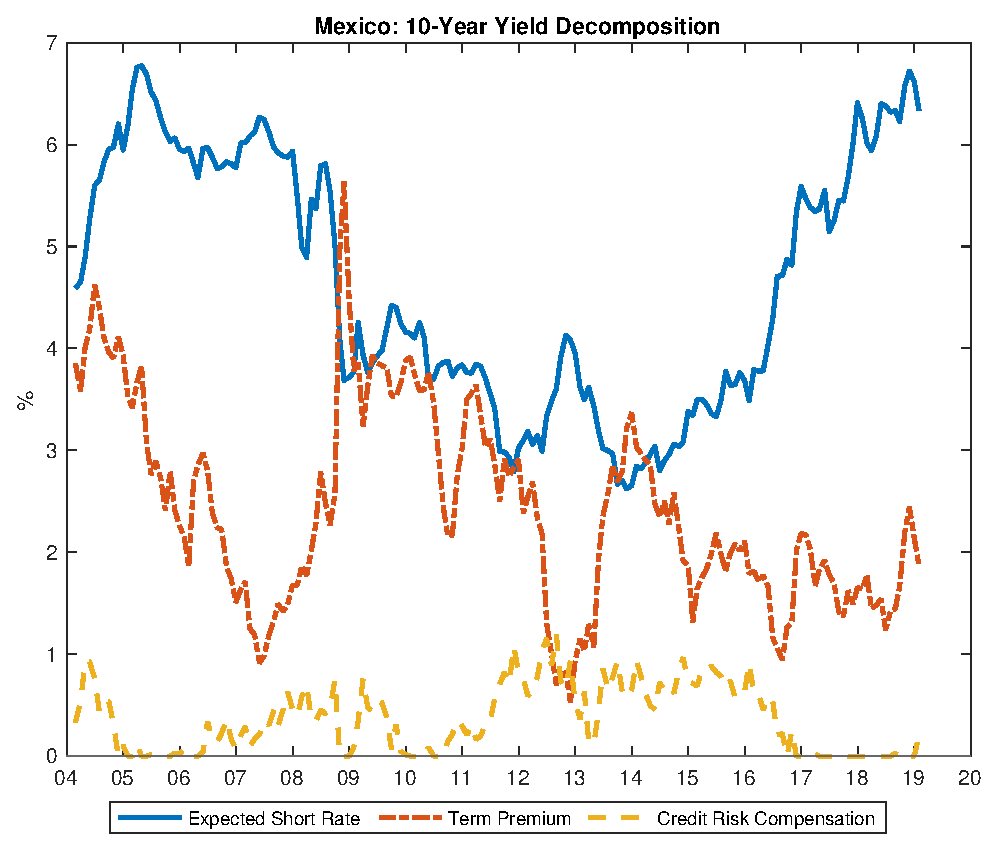
\includegraphics[trim={0cm 0cm 0cm 0cm},clip,width=0.85\textwidth,height=0.9\textheight]{../Figures/Estimation/MX_dcmp}
\end{center}
\end{frame}


\begin{frame}
	\frametitle{U.S. Monetary Policy Spillovers}
	\begin{enumerate}
		\item EM yields' response is \alert{economically significant}, yet \alert{delayed} %over days
		\begin{itemize}
			\item Response in EM slower than in U.S.
			\newline
		\end{itemize}
		
		
		\item \alert{All three} components react to U.S. monetary policy % shocks <2->
		\begin{itemize}
			\item EM central banks expected to follow Fed's monetary stance
			\item EM term premia response similar to AE term premia
			\item Fiscal implications in EM of U.S. monetary policy
			\newline
		\end{itemize} 
	
		\item Unconventional policies \alert{limit} EM monetary autonomy along curve % yield <3>
		\begin{itemize}
			\item Global financial cycle more relevant at the long end
		\end{itemize}
	\end{enumerate}
\end{frame}
\note{The response amplify over the month following the shock.}
\note{This delayed response is consistent with the evidence for the US, which has been attributed to a portfolio rebalancing channel and slow-moving capital.}
\note{However, I find that the effects last longer in EM relative to the U.S.}

\note{All 3 components react giving rise to...}
\note{I find that EM CBs don't counteract the monetary stance in the US but that investors expected them to follow the Fed. If the Fed loosens or tightens financial conditions, EM CBs will follow.}

\note{Finally, I find that since the GFC the GFCy -global comovement of asset prices- is stronger at the long end of the EM YC -LT yields comove more than ST ones- which limits the influence that EM CBs can exert over their local YC.}

%\begin{frame}[label=LitReview]
%	\frametitle{Related Literature}
%	
%	\alert{Synthetic yields} and covered interest rate parity deviations
%	\begin{itemize}
%		\item {\scriptsize \cite{DuSchreger:2016JoF}; \cite*{DuImSchreger:2018JIE}; \cite*{DuTepperVerdelhan:2018}}
%	\end{itemize}
%
%	\alert{Sovereign default} in EM local currency bonds
%	\begin{itemize}
%		\item {\scriptsize \cite{ReinhartRogoff:2011}; \cite{DuSchreger:2016JoF}; \cite{ErceMallucci:2018}; \cite{OttonelloPerez:2019}}
%	\end{itemize}
%	
%	\alert{Global financial cycle}
%	\begin{itemize}
%		\item {\scriptsize \cite{Rey:2013}; \cite{Turner:2014}; \cite{Obstfeld:2015}; \cite{Kalemli-Ozcan:2019}; \cite{KolasaWesolowski:2020}}
%	\end{itemize}
%	
%	\alert{Spillovers} of U.S. monetary policy to EM yields
%	\begin{itemize}
%		\item {\scriptsize \cite{HausmanWongswan:2011}; \cite*{BowmanLondonoSapriza:2015}; \cite*{CurcuruKaminLiRodriguez:2018}; \cite*{Albaglietal:2019}; \cite*{ACDM:2019}}
%	\end{itemize}
%\end{frame}
%\note{Paper related to different branches in the literature.} %However, I will not spend time on them. I will better make references in the relevant parts of the presentation.
%\note{In summary, the literature on term structures of emerging market yields has not examined credit risk systematically, it uses a two-part decomposition, which implicitly treats EM as AE.}
%\note{The analysis of spillovers using yield decompositions has mainly focused on AE and, again, when EM are included, they are treated as AE.}
%
%
%\section{Yield Curves}
%
%
%\begin{frame}
%\frametitle{Nominal Yield Curves}
%
%	 Bloomberg Fair Value par yield curves \(\rightarrow\) Zero-coupon yield curves (\(\yLCnom\))
%	\begin{itemize}
%		\item But \alert{credit risk} in \(\yLCnom\) %LC nominal yields of EM
%	\end{itemize}
%	
%	\textbf{Approach}: \alert{Synthetic} LC yields (\(\yLCsynt\)) as \textit{free of credit risk}
%	\begin{itemize}
%		\item Swap U.S. Treasury yields into LC using currency derivatives
%	\end{itemize}
%	
%	\textbf{Assumption}: Frictionless financial markets \citep{DuSchreger:2016JoF}
%	\begin{itemize}
%		\item Arbitrageurs have access to U.S. and LC bonds
%		\item Derivatives have no counterparty risk
%		\item U.S. yields are free of default risk
%	\end{itemize}
%	
%%	Why not CDS (credit default swaps)?
%\end{frame}
%\note{Sovereign debt of AEs is considered free of credit risk.}
%%\note{Synthetic instead of nominal yields.}
%\note{Under this approach, US YC used as a benchmark for all EMs.}
%\note{An alternative approach to synthetic yields is to use CDS, however they do not adequately characterize LC credit risk because defaults on LC bonds governed under domestic law do not trigger CDS payouts.}
%\note{This approach assumes frictionless financial markets.}
%\note{There circumstances in which these assumptions are violated, even the last one. But \cite{DuSchreger:2016JoF} show it is a \alert{useful benchmark}.}
%%\note{Broad perspective on credit risk, i.e. not receiving promised payments: EMs can change the law + Suspension of currency convertibility + Capital controls + Actual default.}
%%\note{BFV curves are par yield curves provided by Bloomberg on a daily basis for different maturities. To obtain the implied zero-coupon curves, the yields are converted into discount factors, which are then used to estimate the parameters of the Nelson-Siegel-Svensson model.}
%%\note{CDS is a financial derivative that enable investors to swap credit risk.}
%
%
%\begin{frame}[label=Synthetic]
%\frametitle{Synthetic Yield Curves}
%%\vspace{-1cm}
%\begin{equation*} \label{eq:uLCsynt}
	\eqyLCsynt
\end{equation*}
%%\vspace{-0.5cm}
%
%	\(\yLCsynt\): \(\tnr\)-period zero-coupon \textit{synthetic} yield of a country in LC at time $t$
%	
%	\(\yUS\): \(\tnr\)-period zero-coupon yield of the U.S. in USD at time \(\idxt\)
%	
%	\(\fwdprm\): \(\tnr\)-period foreign exchange \alert{forward premium} from USD to LC at time \(\idxt\)
%%	\begin{itemize}
%%		\item Currency forwards (\(< 1\) year) and cross-currency swaps (\(\geq 1\) year)
%%	\end{itemize}
%	
%	\begin{itemize}
%		\item \alert{\(< 1\) Year}: Currency forwards
%		\[(forward_{t,\tnr} - spot_{t})/\tnr\]
%		\item \alert{\(\geq 1\) Year}: Cross-currency swaps %Fixed-for-fixed 
%		%	\iftoggle{long}{\pause}{}
%		\begin{itemize}
%			\item Cross-currency basis swaps
%			\item Interest rate swaps
%		\end{itemize}
%	\end{itemize}
%%	\begin{textblock*}{3cm}(.92\textwidth,0.74\textheight)
%%		\hyperlink{FwdPrm}{\beamergotobutton{FP}}
%%	\end{textblock*}
%\end{frame}
%\note{FP compensates for the depreciation of the LC.}
%\note{For maturities of less than one year, FP is calculated as the annualized difference between the forward and the spot exchange rates.}
%\note{For maturities equal or larger than one year, FP is calculated using cross-currency swaps because outright forwards are less liquid.}
%\note{Notice that the nominal YC is not needed to construct the synthetic YC.}
%
%\note{Today I can lock in a risk-free investment in LC by exchanging LC for USD, investing those USD in Tresuaries and enter into a forward contract agreeing to sell USD for LC in the future. Once I receive the payment from Treasuries, I exchange it back into LC.}
%\note{Fixed-for-fixed XCS not directly traded in the market but they can be constructed.}
%\note{CCS and IRS are liquid and collateralized. Bilateral counterparty risk is small.}
%
%
%\begin{frame}[label=DevCIP]
%\frametitle{Deviations from CIP (Covered Interest Parity)}
%%\vspace{-1cm}
%\[\eqCIPdevDS\]
%
%	Measures:
%	\begin{itemize}
%		\item \alert{Sovereign credit risk} in EM
%		\item[] {\small \cite{DuSchreger:2016JoF}} 
%		\item \alert{Convenience yield} for advanced economies (AE)
%		\item[] {\small \cite*{DuImSchreger:2018JIE}} 
%		\item Financial market \alert{frictions} for banks 
%		\item[] {\small \cite*{DuTepperVerdelhan:2018}}
%	\end{itemize}
%
%	\textbf{Here}: Emphasis on \(\yLCsynt\)
%\end{frame}
%\note{Diff b/w nominal and synthetic measures CIP deviations in government yields.}
%\note{The interpreation of the spread depends on the context.}
%\note{For EM, pread b/w LCNOM and LCSYNT is the CRC.}
%\note{Correlation b/w CIP dev and CDS is high for EMs but not for AEs.}
%\note{While the literature has focused on the spread, I focus on the synthetic yields themeselves.}
%
%
%\begin{frame}
%\frametitle{Data}
%	\alert{15 EM} countries:
%	\begin{itemize}
%%		\item[] {\scriptsize BRL, COP, HUF, IDR, ILS, KRW, MYR, MXN, PEN, PHP, PLN, RUB, THB, TRY, ZAR}
%		\item {\small Brazil, Colombia, Hungary, Indonesia, Israel, Korea, Malaysia, Mexico, Peru, Philippines, Poland, Russia, Thailand, Turkey, South Africa}
%	\end{itemize}
%	%	\begin{itemize}
%	%		\item \scriptsize \alert{10 AEs}: AUD, CAD, CHF, DKK, EUR, GBP, JPY, NOK, NZD, SEK
%	%	\end{itemize}
%%	\iftoggle{struct}{\item<2->}{\item} 
%	
%	\alert{Daily} data starting in January 2000 to January 2019
%%	\iftoggle{struct}{\item<3->}{\item}
%	
%	Maturities (in years): 0.25, 0.5, 1, 2, \ldots, 10
%%	\iftoggle{struct}{\item<4->}{\item}
%	
%	Sources for \alert{synthetic} yields:
%	\begin{itemize}
%%		\iftoggle{struct}{\item<5->}{\item}
%		\item $\yUS$: \citet*{GSW:2007}; CRSP Risk-Free Rates
%%		\vspace{-0.1cm}
%%		\iftoggle{struct}{\item<6->}{\item}
%		\item $\fwdprm$: Bloomberg; Datastream
%	\end{itemize}
%\end{frame}
%\note{Starting dates vary by country.}
%\note{Longer series desirable to pin down TP since unobserved. But at least 10 years of data, which is a reasonable sample size for the estimation of the model.}
%\note{Bonds\(>10Y\) tend to have less history and be less liquid, including the swaps used to construct the synthetic YC.}
%
%\note{The construction of the synthetic yields uses the dataset developed by GSW, which adecuately captures the USYC for maturities larger than 1Y.}
%\note{For 3M and 6M I use data from CRSP (which is more robust at the short end).}
%
%\note{Results are compared against those obtained for 10 AEs.}
%%\note{Reasons for use monthly: VAR is a good approximation for monthly, adequate frequency if want to use macro data.}
%%\note{Consensus Economics provides long-horizon forecasts for consumer inflation and real GDP growth but not for policy rates.}
%
%
%\begin{frame}
%	\frametitle{Descriptive Statistics}
%	\begin{figure}[!htbp]
%		\begin{center} % trim removes: left, down, right, top
%			\includegraphics[trim={2.5cm 7.5cm 2.5cm 10cm},clip, width=0.95\textwidth,height=1.05\textheight]{../Tables/yldcrvstats.pdf}
%			\par\end{center}
%	\end{figure}
%\end{frame}
%\note{Table reports descriptive statistics for different tenors of the nominal and synthetic YC for the EM and includes those from AE for comparison.}
%\note{YCs exhibit standard properties such as an upward slope.}
%\note{In general interest rates in EM are higher than in AE, the table reflects that.}
%
%\note{For instance, the level and the volatility of EM curves are larger than those of AE.} 
%\note{Also, the short end of their curves is more volatile than the long end, particularly so for the synthetic curve.}
%\note{Higher volatility at ST makes the model's fit at ST harder. Don't affect the results b/c the analysis focuses on the 2Y and 10Y.}
%\note{10 AEs: AUD, CAD, CHF, DKK, EUR, GBP, JPY, NOK, NZD, SEK}
%
%
%\section{Affine Term Structure Model}
%
%\begin{frame}[label=ATSMsummary]
%\frametitle{Model Overview}
%	
%	Standard discrete-time nominal affine term structure model
%	\begin{itemize}
%		\item Assumes default-free bonds \(\rightarrow\) \alert{Synthetic} yields (\(\yLCsynt\)) for EM
%	\end{itemize}
%	
%	Intuition:
%	\begin{itemize}
%		\item Yields driven by pricing factors \(\Xvars\)
%		\item Dynamics of pricing factors (\(\Pmeasure\) and \(\Qmeasure\) measures)
%		\item No-arbitrage restrictions ensure consistency % in cross section / time series of yields
%%		\item Yields are affine functions of the pricing factors
%	\end{itemize}
%	
%	Model \alert{augmented} with survey data
%	
%	\begin{textblock*}{3cm}(0.08\textwidth,1.05\textheight)
%	\hyperlink{AssetPricing}{\beamergotobutton{Asset Pricing}}
%	\end{textblock*}
%	\begin{textblock*}{3cm}(0.23\textwidth,1.05\textheight)
%		\hyperlink{SDF}{\beamergotobutton{SDF}}
%	\end{textblock*}
%	\begin{textblock*}{3cm}(0.32\textwidth,1.05\textheight)
%		\hyperlink{BondPrices}{\beamergotobutton{Bond Prices}}
%	\end{textblock*}
%	\begin{textblock*}{3cm}(0.46\textwidth,1.05\textheight)
%		\hyperlink{SvyAugModel}{\beamergotobutton{Augmented Version}}
%	\end{textblock*}
%\end{frame}
%\note{ATSM standard tool to estimate dynamics of risk-free \alert{nominal} yield curves.}
%\note{It assumes yields are risk-free.}
%\note{For EM, synthetic curve better aligns with the risk-free assumption.}
%\note{By decomposing synthetic yields into YP and TP allows me to decompose nominal into 3 parts.}
%%\note{The coefficients are functions of the maturity of the bond and the coefficients that determine the stochastic processes that drive the state variables.}
%
%
%\begin{frame}[label=Components]
%\frametitle{EM Yield Decomposition}
%
%Fitted \alert{synthetic} yields
%\begin{equation*}
	\yZeroQ = - \frac{\affineA}{\tnr} - \frac{\affineB}{\tnr} \Xvars = \affineA^{\Qmeasure} + \affineB^{\Qmeasure} \Xvars,
\end{equation*}
%
%Average expected future short rate %(\(\lambdazero = \lambdaone = 0\)) as if investors were risk-neutral
%\begin{equation*}
	\yZeroP = \affineAP + \affineBP \Xvars,
	%\yZeroP = - \frac{\affineA}{\tnr} - \frac{\affineB}{\tnr} \Xvars = \affineA^{\Pmeasure} + \affineB^{\Pmeasure} \Xvars,
\end{equation*}
%
%Term premium
%\begin{equation*} \label{eq:uTPatsm}
	\eqTP
\end{equation*}

% \termprm = \yZeroQ - \yZeroP
%
%Credit risk compensation
%\[\CIPdev = \yLCnom - \yZeroQ \] % \geq 0
%
%\end{frame}
%\note{Once parameters estimated, decompose yields.}
%
%
%\begin{frame}
%\frametitle{Weak Identification}
%
%Yields \alert{accurately} identify \{\(\XmuQ, \XPhiQ\)\}, yet \{\(\XmuP, \XPhiP\)\} \alert{poorly} identified
%\begin{itemize}
%	\item Bond yields are persistent
%	\item Unstable yield decompositions
%\end{itemize}
%
%\textbf{Solutions}: Survey data, parameter restrictions, bias-corrected estimators
%
%Surveys provide \alert{robust} decompositions of AE yields \citep{Guimaraes:2014}
%\begin{itemize}
%	\item Important for EM yields due to small sample sizes
%\end{itemize}
%%Most variability attributed to fluctuations in term premium
%% Overestimates stability of expected path of short rate
%
%\end{frame}
%\note{Only ZC bond yields are needed to estimate ATSM parameters.}
%\note{Poorly identified parameters under the \(\Pmeasure\) measure result in unstable yield decompositions.}
%\note{TP is an unobserved variable.}
%\note{That is why it is desirable to have long time series for the estimation.}
%\note{Solutions proposes include complementing data from yields with surveys on interest rate forecasts, especially long-term ones.}
%\note{... Surveys anchor long run mean of interest rates.}
%
%\note{Overestimates stability of expected path of short rate}
%%\note{Surveys are an effective solution to obtain robust decompositions of the yield curve \citep{Guimaraes:2014} 
%
%\begin{frame}[label=SCBP]
%\frametitle{Survey Data}
%
%No data on long-term forecasts for EM short rates
%
%Implied forecast for EM short rates using existing data %on long-term forecasts
%\begin{itemize}
%\item \alert{EM inflation} expectations: 5 years ahead and long-term
%\begin{itemize}
%	\item Twice a year from Consensus Economics (CE)
%\end{itemize}
%
%\item Implied long-term expectations of \alert{U.S real interest rate} 
%\begin{itemize}
%\item T-bill rate, CPI inflation from Survey of Professional Forecasters (SPF)
%%\item Compared against TIPS yields
%\end{itemize}
%\end{itemize}
%
%\begin{equation*} \label{eq:uRrt}
	\eqrrt 
\end{equation*}
%
%\begin{textblock*}{3cm}(.9\textwidth,1.05\textheight)
%	\hyperlink{YldCBP}{\beamergotobutton{Implied Forecasts}}
%\end{textblock*}
%\end{frame}
%\note{No data.}
%\note{Inferred from existing data using the Fisher equation and treating EMs as small open economies, which implies that the global real rate is determined abroad.}
%\note{This requires forecasts for inflation in each EM and for the global real interest rate.}
%\note{Inflation forecasts from CE, which are published twice a year.}
%\note{U.S. real rate serves as a proxy for the global real rate and is derived using forecasts for the T-bill rate and CPI inflation from SPF.}
%\note{This is done using 5Y ahead forecasts and long-term forecasts (b/w 5Y and 10Y ahead).}
%
%\note{I compare them also against the real yields from TIPS and against an alternative approach using Taylor-rule type regressions, which also use forecasts for real GDP. The results are also comparable.}
%
%
%\begin{frame}
%\frametitle{Model Estimation}
%
%%	\item Use \cite*{JSZ:2011} normalization of the model %: \(\Pmeasure \perp \Qmeasure\) % likelihood functions
%Estimate parameters by MLE with \alert{monthly} data
%\begin{itemize}
%\item \cite*{JSZ:2011} normalization
%\end{itemize}
%%	\item Estimate \(\Pmeasure\) parameters by OLS
%%	\item Estimate \(\Qmeasure\) parameters by MLE
%
%Estimate survey-augmented model by Kalman filter (missing data)
%\begin{itemize}
%\item Surveys as \alert{`noisy'} expectations measures \citep{KimOrphanides:2012}
%\end{itemize}
%
%Standard errors by delta method
%
%Estimate \alert{daily} pricing factors
%
%\end{frame}
%\note{End-of-month data. Since surveys twice a year, they treated as mising data in non-release dates so model estimated by KF. with initial values obtained by estimating the model using only data on synthetic yields.}
%\note{Surveys contain useful information and help in anchoring the model to the reality in each country but they are not a panacea, so they are treated as `noisy' measures of expectations by using a conservative value for their standard devaition.}
%\note{Finally, I use the parameters estimated with monthly data to estimate the pricing factors at the daily frequency. This allows me to decompose the yields at the daily frequency, which is needed to analyze the spillovers from US MP.}
%
%\note{At the daily frequency there is noise in yield data that can undermine the estimation.}
%
%
%\section{EM Yield Decomposition}
%
%
%\begin{frame}[label=ModelFit]
%%	\frametitle{Model Fit}
%\vspace{0.2cm}
%\begin{center}							% center the figure inside the minipage
%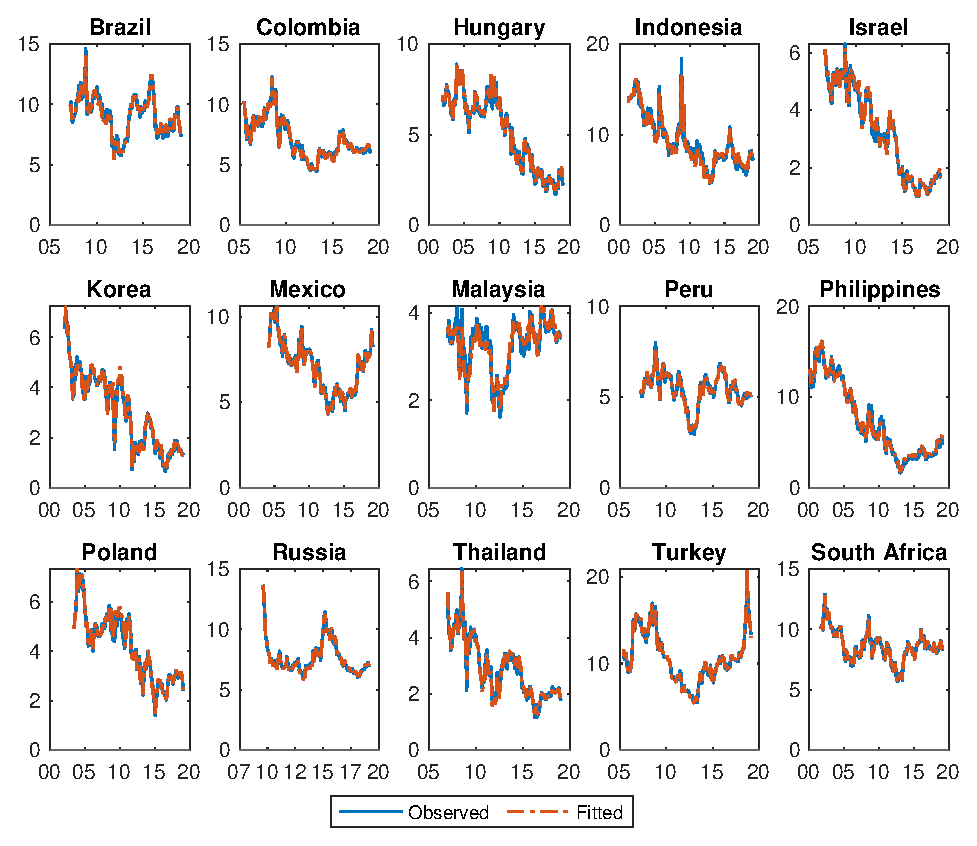
\includegraphics[trim={0cm 0cm 0cm 0cm},clip,height=0.95\textheight,width=\linewidth]{../Figures/Estimation/s_ylds_bsl_yQ.eps} \\
%\end{center}
%\begin{textblock*}{15cm}(2.5mm,3mm)
%	\textbf{10Y}
%\end{textblock*}
%\end{frame}
%\note{Figure 3 illustrates the fit of the model for the synthetic yields.}
%\note{In general, the model fits the data reasonably well.}
%
%
%\begin{frame}
%\frametitle{Average EM Yield Curve Decomposition}
%\vspace{5pt}
%\begin{center}
%	\includegraphics[trim={0.1cm 0.1cm 0.1cm 0cm},clip,width=0.85\textwidth,height=0.85\textheight]{../Figures/Slides/Yield_Dcmp_EM.png}
%\end{center}
%\end{frame}
%\note{Figure summarizes the decomposition across EM.}
%\note{Describe colors.}
%\note{On average, ESR explains most of the variability in yields; but their importance decreases with maturity.}
%\note{The relevance of the term premium increases with maturity.}
%\note{CRC remains stable across maturities.}
%\note{Broadly speaking the 10Y 7 = 4 + 2 + 1 or 60-30-10 percent.}
%
%
%\begin{frame}[label=YldDcmp]
%%	\frametitle{Decomposition of EM Nominal Yields}
%\begin{center}							% center the figure inside the minipage
%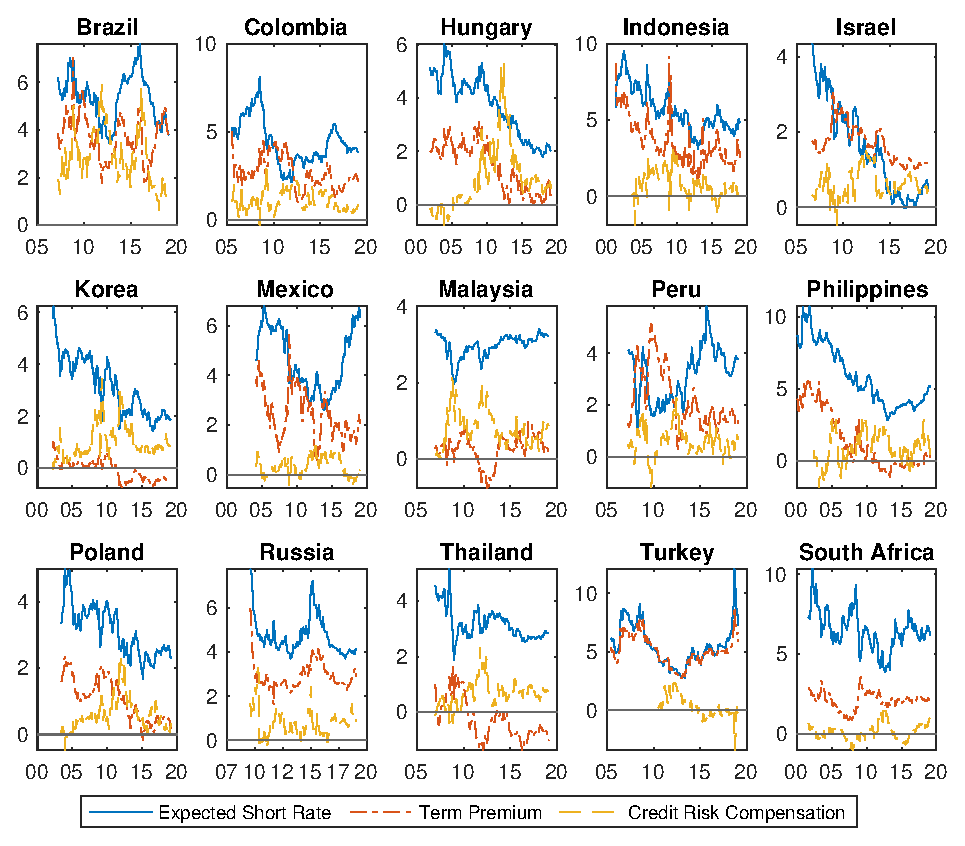
\includegraphics[trim={0cm 0cm 0cm 0cm},clip,height=0.95\textheight,width=\linewidth]{../Figures/Estimation/ny_dcmp.eps} \\
%\end{center}
%\begin{textblock*}{15cm}(2.5mm,3mm)
%	\textbf{10Y}
%\end{textblock*}
%\begin{textblock*}{3cm}(.51\textwidth,1.08\textheight)
%\hyperlink{tpCI}{\beamergotobutton{Term Premia}}
%\end{textblock*}
%\begin{textblock*}{5cm}(.725\textwidth,1.08\textheight)
%\hyperlink{crcCI}{\beamergotobutton{Credit Risk Compensation}}
%\end{textblock*}
%\end{frame}
%\note{Dynamics of TP and LCCS important drivers of EM bond yields.}
%\note{TP plays a relatively bigger role, in general.}
%\note{The results for individual countries are consistent with their particular circumstances: MXN and HUF.}
%\note{There is a downward trend in EM TP, which consistent w/ the evidence for AE.}
%\note{Since 2011 there has been strong demand for LC bonds in Asia, which partly explains TP < 0 seen in Asian countries.}
%
%\note{TP decline due to: international investors, US UMP.}
%%\note{USTP increased around the onset of the Great Recession (September 2008), the taper tantrum (June 2013), and the 2016 U.S. presidential election (November 2016), while it declined after the first unexpected announcement of the QE program by the Fed (March 2009).}
%%\note{Common explanations for the decline in the USTP include an increased demand of U.S. assets by global investors and the effects of the UMP of the Fed.}
%%\note{Explanation for change in sign (Campbell, Sunderam \& Viceira (2016)): TP < 0 is explained by the flip in the sign of the correlation between stocks and bonds -bonds hedge stocks-.}
%%\note{Events: GR, TT, US election, 2009 QE1.}
%
%
%\begin{frame}[label=yPscbp]
%%	\frametitle{Components: Expected Future Short Rate}
%\vspace{0.1cm}
%\begin{center}							% center the figure inside the minipage
%	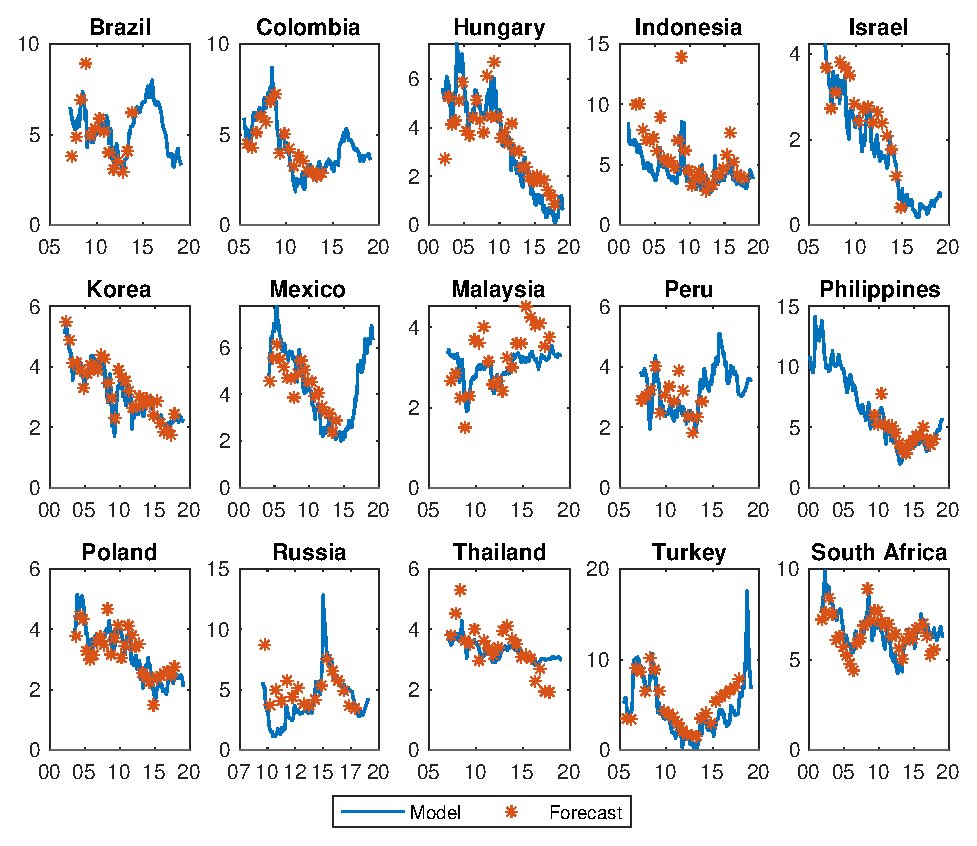
\includegraphics[trim={0cm 0cm 0cm 0cm},clip,height=0.95\textheight,width=\linewidth]{../Figures/Estimation/bsl_yP_scbp.eps} \\
%\end{center}
%\begin{textblock*}{15cm}(2.5mm,3mm)
%	\textbf{10Y}
%\end{textblock*}
%%\begin{textblock*}{5cm}(0.97\textwidth,1.07\textheight)
%%	\hyperlink{rrtLT}{\beamergotobutton{Real Rates}}
%%\end{textblock*}
%\end{frame}
%\note{D-S have studied CRC, it is highly correlated with CDS.}
%\note{10Y expected future short rate tracks the (implied) long-term
%interest rate forecasts reasonably well.}
%
%
%\begin{frame}[label=tpUCSV]
%\frametitle{Term Premium and Inflation Uncertainty}
%
%Term premium compensates for \alert{inflation uncertainty} \citep{Wright:2011}
%%In advanced economies related to inflation uncertainty \citep{Wright:2011} % in advanced economies
%
%Inflation higher and \alert{more volatile} in EM than AE \citep{HaKoseOhnsorge:2019}
%\newline
%
%Is inflation uncertainty relevant for EM term premia?
%\begin{equation*} \label{eq:uPanelUCSV}
	\eqpanelUCSV ,
\end{equation*}
%
%\(\sigma^{\pi}_{\idxspnl}\) of \(\pi\) permanent component in UCSV model \citep{StockWatson:2007}
%
%\end{frame}
%
%
%\begin{frame}
%\frametitle{EM Term Premia and Inflation Uncertainty}
%%	\setbeamercolor{background canvas}{bg=}
%%	\includepdf[pages={1}]{../Tables/tpucsv.pdf}
%\vspace{-0.8cm}
%\begin{figure}[!htbp]
%\begin{center} % trim removes: left, down, right, top
%\includegraphics[trim={2.5cm 6cm 2.5cm 7cm},clip, width=1\textwidth,height=0.95\textheight]{../Tables/tpucsv.pdf}
%\par\end{center}
%\end{figure}
%\end{frame}
%\note{STD of the permanent is associated with EM TP and the effect increases with maturity.}
%\note{The result becomes stronger after controlling for the business cycle.}
%\note{Even though econometric problems, results aligned with the view that EM TP compensate investors for bearing inflation uncertainty.}
%
%
%\section{U.S. Monetary Policy Spillovers}
%
%\begin{frame}
%\frametitle{The Yield Curve Channel}
%\alert{Long-term yields} influenced by global forces
%\begin{itemize}
%	\item Global financial cycle \citep{Rey:2013}
%\end{itemize}
%
%\alert{Unconventional} monetary policies abroad affect EM yields
%\begin{itemize}
%	\item Long-term via the term premium \citep{Turner:2014}
%	\item Short-term via risk spillovers \citep{Kalemli-Ozcan:2019} 
%\end{itemize}
%
%EM \alert{monetary autonomy}:
%\begin{itemize}
%	\item Declines along the yield curve \citep{Obstfeld:2015}
%	
%%	\begin{itemize}
%%		\item 
%%	\end{itemize}
%\end{itemize}
%\end{frame}
%\note{GFCy: fluctuations in financial activity on a global scale.}
%\note{It is generally thought that CBs exert control on the ST rate and financial markets transmit the stance to LT.}
%
%
%\begin{frame}
%\frametitle{Implications of Yield Curve Channel}
%
%Long-term EM yields \alert{comove more} than short-term ones
%%\begin{itemize}
%%\item Rolling correlations % Connectedness index \citep{DieboldYilmaz:2014}
%%\end{itemize}
%
%\alert{Direct} relationships at different maturities
%\begin{itemize}
%\item U.S. term premium \(\rightarrow\) EM term premium
%\item U.S. expected future short rates \(\rightarrow\) EM expected future short rates
%\end{itemize}
%
%\alert{Cross} relationships at the short end
%\begin{itemize}
%\item U.S. term premium \(\rightarrow\) EM expected future short rates
%\end{itemize}
%
%\end{frame}
%\note{Cross effect at 2Y maturity.}
%
%%\begin{frame}[label=DYindex]
%%\frametitle{EM Yields Comovement}
%%\begin{figure}[!htbp]
%%\begin{center} % trim removes: left, down, right, top
%%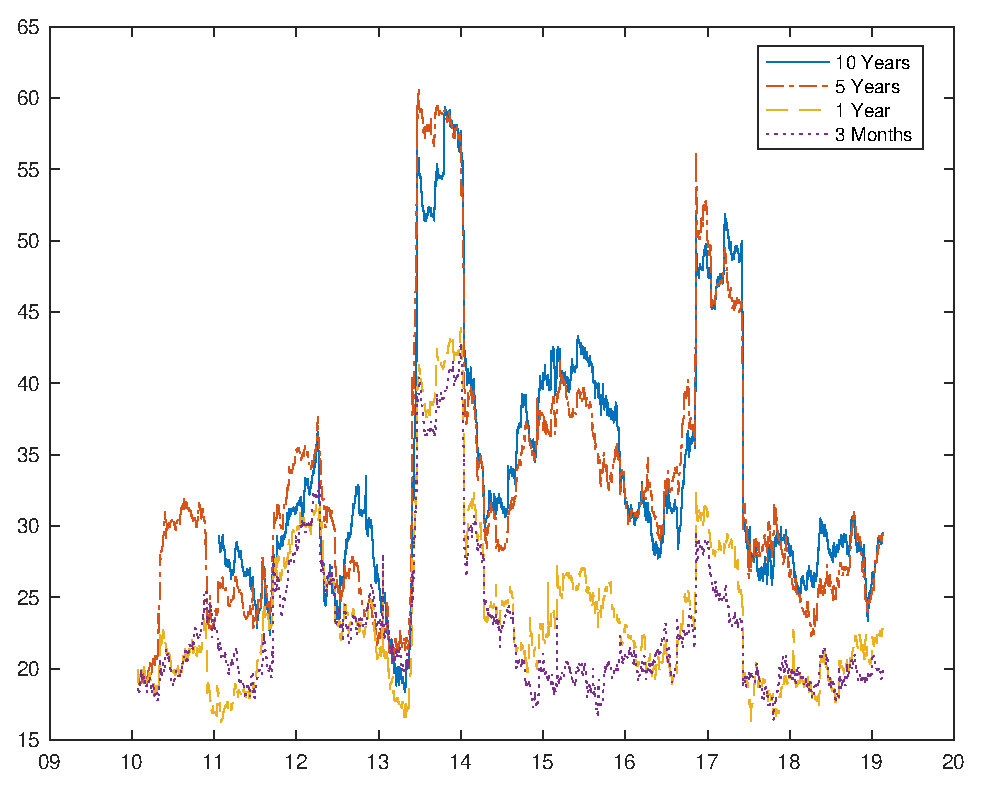
\includegraphics[trim={0cm 0cm 0cm 0cm},clip,height=0.8\textheight,width=0.85\linewidth]{../Figures/Estimation/dy_index_dn_data.eps}
%%\par\end{center}
%%\end{figure}
%%\begin{textblock*}{10cm}(45mm,83mm)
%%\footnotesize Connectedness Index \citep{DieboldYilmaz:2014}
%%\end{textblock*}
%%\begin{textblock*}{5cm}(1.02\textwidth,0.55\textheight)
%%	\hyperlink{RollingCorr}{\beamergotobutton{Rolling Corr.}}
%%\end{textblock*}
%%\end{frame}
%
%\begin{frame}[label=RollingCorr]
%\frametitle{EM Yields Comovement}
%\begin{figure}[!htbp]
%	\begin{center} % trim removes: left, down, right, top
%		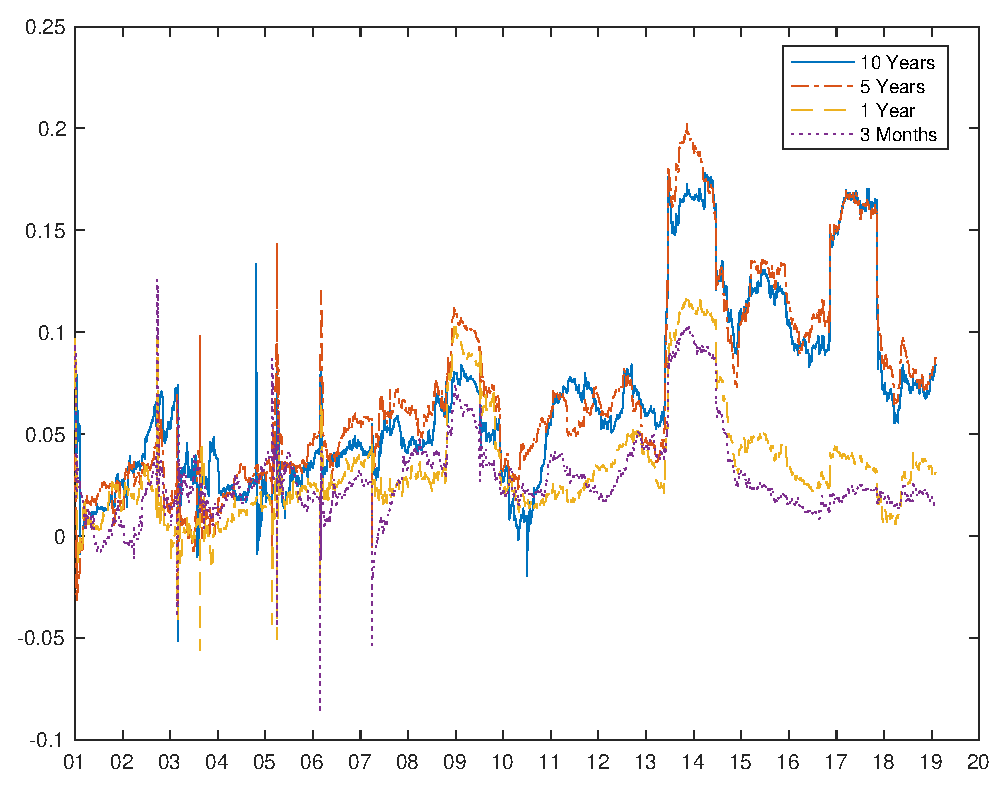
\includegraphics[trim={0cm 0cm 0cm 0cm},clip,height=0.8\textheight,width=0.85\linewidth]{../Figures/Estimation/rolling_dn_data.eps}
%		\par\end{center}
%\end{figure}
%\begin{textblock*}{10cm}(67.5mm,83mm)
%	\footnotesize Rolling Correlations
%\end{textblock*}
%\begin{textblock*}{5cm}(1.02\textwidth,0.6\textheight)
%	\hyperlink{DYindex}{\beamergotobutton{D-Y Index}}
%\end{textblock*}
%\end{frame}
%
%
%\begin{frame}
%\frametitle{Is There A Yield Curve Channel?}
%%\begin{itemize}
%%	\item Panel regression:
%%\vspace{-1cm}
%\begin{equation*} \label{eq:uPanelDCMP}
	\eqpanelTPreg
\end{equation*}
%%\vspace{-1cm}
%
%\(\yld_{\idxspnl}\): nominal EM yields and their three components
%
%\(\alpha_{i}\): country fixed effects
%
%\(z^{1}_{\idxspnl}\): U.S. yield curve decomposition \citep{KimWright:2005}
%
%\(z^{2}_{\idxspnl}\): Global and domestic drivers
%\begin{itemize}
%	\item VIX, EPU \citep{BakerBloomDavis:2016} \& global activity  \citep{Hamilton:2019} indexes
%	\item Policy rate, inflation, unemployment, exchange rate (standardized) %(LC per USD)
%\end{itemize}
%
%%\end{itemize}
%\end{frame}
%\note{Country FE allow for the possibility that country-specific factors that may affect TP are also correlated with the controls.}
%
%
%\begin{frame}[label=Drivers10Y2Y]
%\vspace{-0.9cm} % \vspace{-2.2cm}
%\begin{center}
%	\begin{tikzpicture}
%	\node (table) at (0,0)
%	{\includegraphics[trim={2cm 6.7cm 2cm 4cm},clip, width=0.95\textwidth,height=1.15\textheight]{../Tables/ycdcmp10y2y.pdf}};
%	% \draw[step=0.5cm,gray,very thin] (-4,-4) grid (6,6);
%	\onslide<2>{
%		\draw[blue,thick] (-0.2,1.24) rectangle (1.2,1.7); %YP10Y
%		\draw[blue,thick] (-0.2,-1.49) rectangle (1.2,-1.02); %YP2Y
%		\draw[orange,thick] (-0.2,0.75) rectangle (1.2,1.21); %CBP10Y
%		\draw[orange,thick] (-0.2,-2) rectangle (1.2,-1.523); %CBP2Y
%	}
%	\onslide<3>{
%		\draw[blue,thick] (2,1.72) rectangle (3.5,2.19); % TP10Y
%		\draw[blue,thick] (2,-1.05) rectangle (3.5,-0.54); %TP2Y
%		\draw[orange,thick] (2,0.23) rectangle (3.5,0.74); % VIX10Y
%		\draw[orange,thick] (2,-2.52) rectangle (3.5,-2); %VIX2Y
%	}
%	\onslide<4>{
%		\draw[blue,thick] (-0.2,1.7) rectangle (1.2,2.2); %TP10Y
%		\draw[blue,thick] (-0.2,-1.05) rectangle (1.2,-0.54); %TP2Y
%		\draw[orange,thick] (-0.2,0.24) rectangle (1.2,0.74); % VIX10Y
%		\draw[orange,thick] (-0.2,-2.52) rectangle (1.2,-2); %VIX2Y
%	}
%	\end{tikzpicture}
%\end{center}
%\begin{textblock*}{5cm}(1.07\textwidth,0.175\textheight)
%	\hyperlink{Drivers10Y}{\beamergotobutton{10Y}}
%\end{textblock*}
%\begin{textblock*}{5cm}(1.07\textwidth,0.525\textheight)
%	\hyperlink{Drivers2Y}{\beamergotobutton{2Y}}
%\end{textblock*}
%\end{frame}
%\note{Response of ESR to CBP is stronger at ST than at LT and is associated with its US counterpart only at the LT -> Monetary autonomy is stronger at the ST than at LT.}
%
%\note{EM TP response to USTP increases with maturity and is positively associated with the Vix only at LT -> USTP and GFCy are more relevant for the LT than for the ST.}
%
%\note{There are risk spillovers to the ESR, they are stronger at the ST than LT and operate through the USTP rather than the VIX.}
%
%\note{All results support the YC channel.}
%\note{However, this specification might be subject to econometric problems such as omitted variables. Moreover, the analysis does not identify USMP shocks and is not suitable to analyze the persistence of the effects.}
%%\note{Higher TP during recessions: high UNE, low IP. Evidence of EM TP countercyclical.}
%%\note{INF erodes value of nominal bonds: in periods of rising INF demand a higher TP.}
%%\note{Higher TP due to FX depreciation in line with risk-taking channel of FX.
%%	Currency depreciation tightens financial conditions, higher sovereign bond spreads.}
%%\note{Effect of the domestic variables in line with findings for AEs. 
%%	Investors demand a higher term premium during recessions, when the unemployment rate increases. This shows evidence of a countercyclical behavior of the TP in EMs.
%%	The positive effect of inflation on the TP conforms with the idea that inflation erodes the value of nominal bonds and so in periods of rising inflation investors demand a higher TP.}
%%\note{A depreciation of the LC is associated with an increase in the TP. This seems counterintuitive since EMs are usually commodity exporters so it appears to contradict the standard trade-channel effect. 
%%	However, it is in line with the risk-taking channel of exchange rates found by \cite{HofmannShimShin:2017}, according to which currency depreciation is associated with tighter financial conditions and increased sovereign bond spreads.}
%
%
%%\begin{frame}[label=Drivers10Y2Y]
%%\vspace{-0.8cm}
%%\begin{figure}[!htbp]
%%	\begin{center} % trim removes: left, down, right, top
%%		\includegraphics[trim={2cm 6.7cm 2cm 4cm},clip, width=0.95\textwidth,height=1.15\textheight]{../Tables/ycdcmp10y2y.pdf}
%%		\par\end{center}
%%\end{figure}
%%\begin{textblock*}{5cm}(1.07\textwidth,0.175\textheight)
%%	\hyperlink{Drivers10Y}{\beamergotobutton{10Y}}
%%\end{textblock*}
%%\begin{textblock*}{5cm}(1.07\textwidth,0.525\textheight)
%%	\hyperlink{Drivers2Y}{\beamergotobutton{2Y}}
%%\end{textblock*}
%%\end{frame}
%
%
%{%
%	\setbeamertemplate{frame footer}{See \cite{Kuttner:2001,GSS:2005a,Swanson:2018,RogersScottiWright:2018}.}
%\begin{frame}
%\frametitle{U.S. Monetary Policy Surprises}
%
%Asset price changes in 2-hour windows around FOMC meetings % since 2000
%%Surprises:
%	\begin{itemize}
%		\item \alert{Target}: federal funds futures contracts
%		\item \alert{Forward guidance}: residual of 8th Eurodollar yield on target surprise
%		\item \alert{Asset purchases}: residual of 10Y Treasury yield on previous surprises % target and forward guidance surprises starting in 2009
%	\end{itemize}
%\begin{center}
%\input{../Figures/MPS/USMPtimeline}
%\end{center}
%%\begin{center}
%%	\includegraphics[trim={0cm 0cm 0cm 0cm},clip,width=0.85\textwidth,height=0.95\textheight]{../Figures/MPS/USMPtimeline}
%%\end{center}
%\end{frame}
%}
%
%\begin{frame}
%\frametitle{Measuring the Effects on EM Yields}
%%\vspace{-1cm}
%Panel local projections:
%\begin{equation*} \label{eq:uPanelLP}
	\eqpanelLP
\end{equation*}	% \ref{eq:nPanelLP}
%%\vspace{-0.7cm}
%\begin{itemize}
%\item \(\yld_{\idxspnl}\): 10Y and 2Y nominal \alert{EM yields} and their \alert{components}
%\item \(\idxh = 0, 1, \ldots, 45\) days
%\item \(\alpha_{\idxh,\idxi}\): country fixed effects
%\item \(\epsilon^{j}_{\idxt}\): \alert{three} types of monetary policy \alert{surprises}
%\item \(\fx_{\idxspnllag}\): one-day lag in the exchange rate
%\end{itemize}
%\end{frame}
%\note{Evidence of delayed response in AE.}
%\note{All responses are assessed relative to a one basis point reduction (an easing) in any of the surprises.}
%\note{The transmission of USMP to EM yields assessed using panel LPs for the daily changes in the yields}
%\note{This allows me not only to capture the response on the day of a surprise but on the following days.}
%
%\note{Large number of daily observations reduces the potential for Nickell bias. Responses are essentially the same when I removed the lag of depvar.}
%
%
%\begin{frame}[label=TargetEM]
%\frametitle{Effects of Target Easing on EM Yields}
%\begin{figure}[!htbp]
%\begin{center} % trim removes: left, down, right, top
%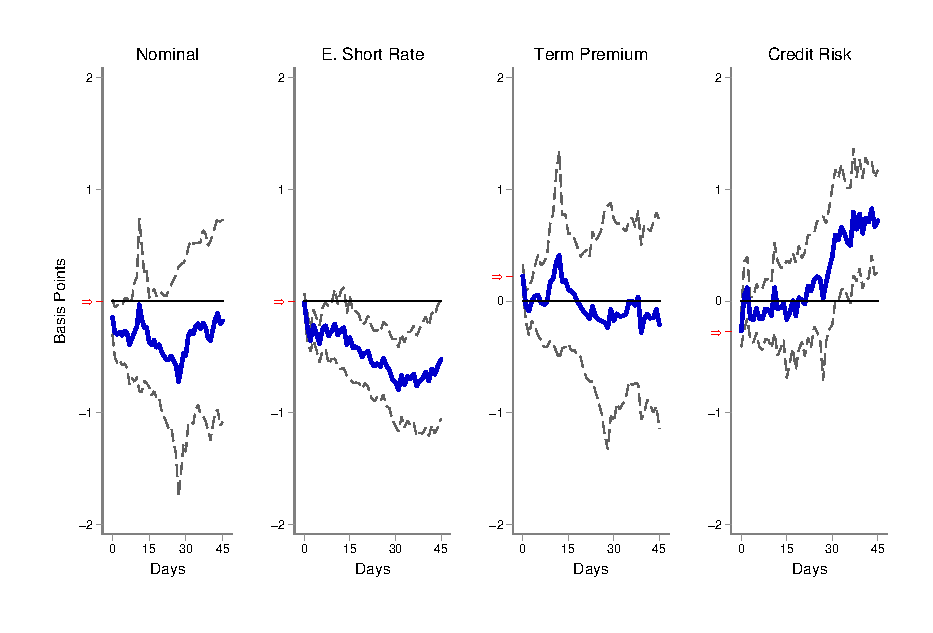
\includegraphics[trim={0cm 0cm 0cm 0cm},clip,height=0.45\textheight,width=0.85\linewidth]{../Figures/LPs/LagDep-FX/Target/EM/TargetEMnomyptpphi120m.eps}
%\par\end{center}
%\end{figure}
%\vspace{-0.5cm}
%\begin{figure}[!htbp]
%\begin{center} % trim removes: left, down, right, top
%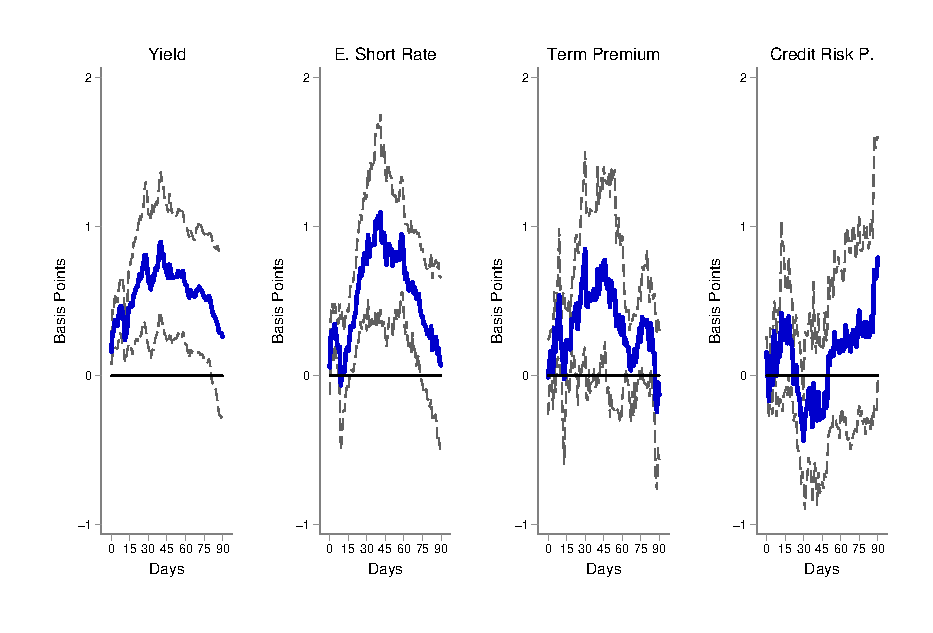
\includegraphics[trim={0cm 0cm 0cm 0.76cm},clip,height=0.45\textheight,width=0.85\linewidth]{../Figures/LPs/LagDep-FX/Target/EM/TargetEMnomyptpphi24m.eps}
%\par\end{center}
%\end{figure}
%\begin{textblock*}{8mm}(10mm,30mm)
%\small \textbf{10Y}
%\end{textblock*}
%\begin{textblock*}{8mm}(10mm,65mm)
%\small \textbf{2Y}
%\end{textblock*}
%\begin{textblock*}{5cm}(1.07\textwidth,0.65\textheight)
%\hyperlink{TargetUS}{\beamergotobutton{US}}
%\end{textblock*}
%\end{frame}
%\note{Responses to a 1 bp easing surprise.}
%\note{Responses of 2Y and 10Y yields and their components.}
%\note{Red arrows show the response on the day of the shock.}
%\note{DK SE, dotted lines are 90\% confidence bands}
%\note{To understand the responses to the shocks one needs to analyze the effect of the shocks on both nominal and the synthetic YCs.}
%
%\note{Following a target easing surprise, both the US and EM YCs steepen.}
%\note{Response builds over time.}
%\note{Investors expect for EM CB to follow the US monetary stance. The effects is stronger at ST.}
%\note{Investors reallocate capital towards US yields and ST EM yields which increases the nominal-synthetic spread at LT.}
%
%
%%\begin{frame}
%%\frametitle{Effects of Target Surprises}
%%\begin{center}
%%\begin{tikzpicture}
%%	\node[anchor=north west,inner sep=0] (image) at (0,0) {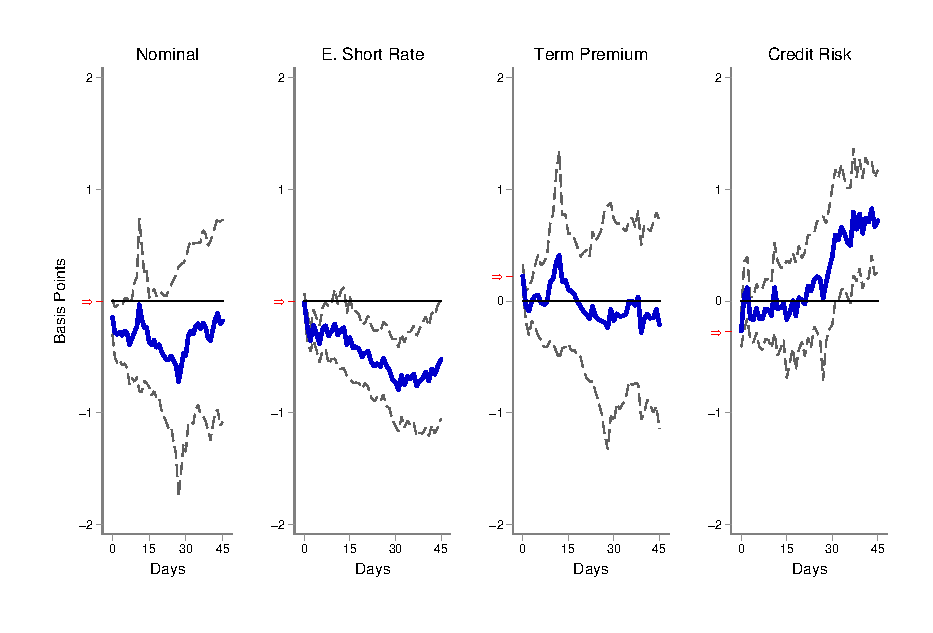
\includegraphics[trim={0cm 0cm 0cm 0cm},clip,height=0.45\textheight,width=0.85\linewidth]{../Figures/LPs/LagDep-FX/Target/EM/TargetEMnomyptpphi120m.eps}};
%%	\begin{scope}[x={(image.south east)},y={(image.north west)}]
%%		\draw[red] (0.3,1) circle (0.1cm);
%%		\draw[blue, semitransparent] (0,0) circle[radius=3pt];
%%		\draw[red] (0.62,0.65) rectangle (0.78,0.75);
%%	\end{scope}
%%%	\draw[red,ultra thick,rounded corners] (7.5,5.3) rectangle (9.4,6.2);
%%\end{tikzpicture}
%%\begin{tikzpicture}
%%	\node[anchor=south west,inner sep=0] (image) at (0,0) {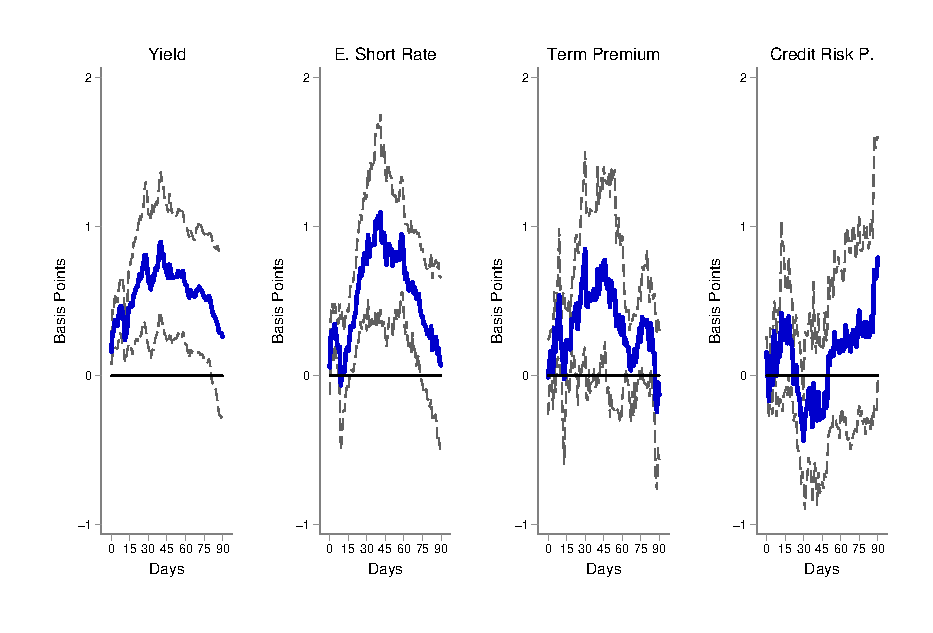
\includegraphics[trim={0cm 0cm 0cm 0.76cm},clip,height=0.45\textheight,width=0.85\linewidth]{../Figures/LPs/LagDep-FX/Target/EM/TargetEMnomyptpphi24m.eps}};
%%%	\draw[red,ultra thick,rounded corners] (7.5,5.3) rectangle (9.4,6.2);
%%\end{tikzpicture}
%%\end{center}
%%\end{frame}
%
%
%\begin{frame}[label=FGEMpre]
%\frametitle{Effects of Forward Guidance Easing on EM Yields: Pre-GFC}
%\begin{figure}[!htbp]
%	\begin{center} % trim removes: left, down, right, top
%		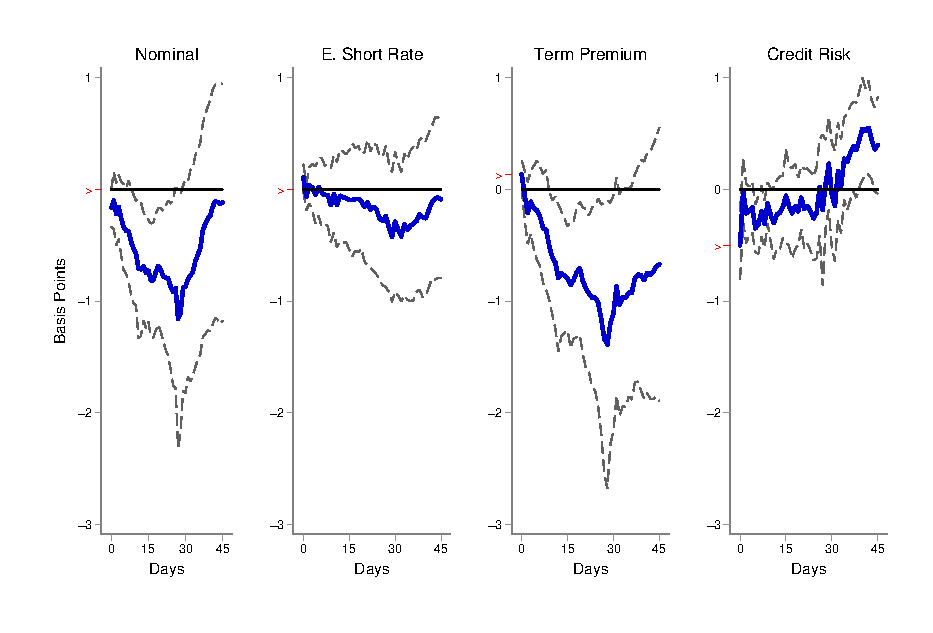
\includegraphics[trim={0cm 0cm 0cm 0cm},clip,height=0.45\textheight,width=0.85\linewidth]{../Figures/LPs/LagDep-FX/Path/EM/PathEMnomyptpphi120mPre.eps}
%		\par\end{center}
%\end{figure}
%\vspace{-0.5cm}
%\begin{figure}[!htbp]
%	\begin{center} % trim removes: left, down, right, top
%		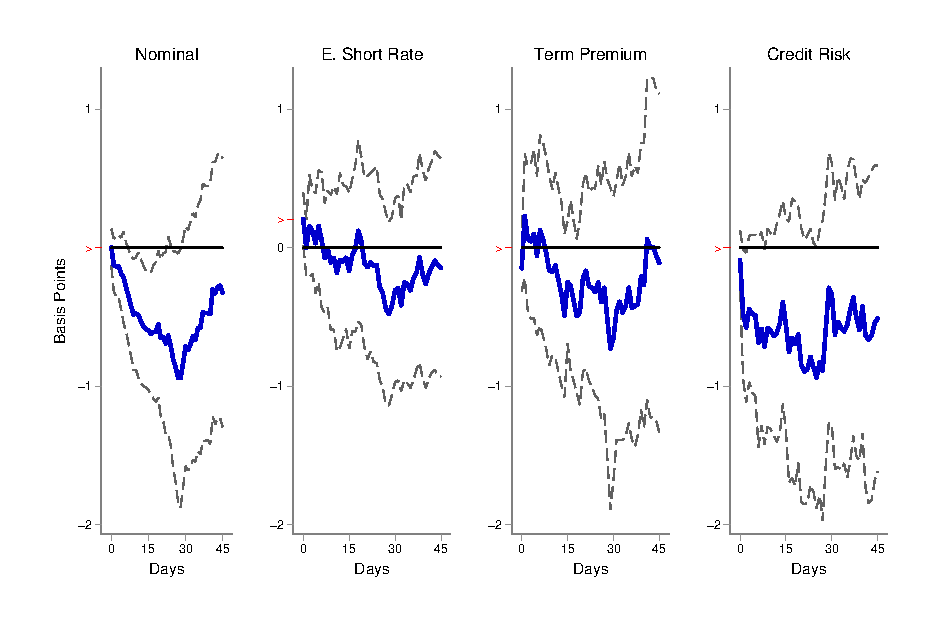
\includegraphics[trim={0cm 0cm 0cm 0.76cm},clip,height=0.45\textheight,width=0.85\linewidth]{../Figures/LPs/LagDep-FX/Path/EM/PathEMnomyptpphi24mPre.eps}
%		\par\end{center}
%\end{figure}
%\begin{textblock*}{8mm}(10mm,30mm)
%	\small \textbf{10Y}
%\end{textblock*}
%\begin{textblock*}{8mm}(10mm,65mm)
%	\small \textbf{2Y}
%\end{textblock*}
%\begin{textblock*}{5cm}(1.07\textwidth,0.65\textheight)
%	\hyperlink{FGUSpre}{\beamergotobutton{US}}
%\end{textblock*}
%\end{frame}
%\note{There is evidence that USMP spillovers to LT yields increased after GFC. So I present the responses before and after the GFC.}
%\note{A FG easing surprise lead to a downward parallel shift in EM YC in the month following the surprise.}
%\note{Response is mainly driven by a parallel decline in TP.}
%\note{Slightly reduces CRC.}
%
%
%\begin{frame}[label=FGEMpost]
%\frametitle{Effects of Forward Guidance Easing on EM Yields: Post-GFC}
%\begin{figure}[!htbp]
%\begin{center} % trim removes: left, down, right, top
%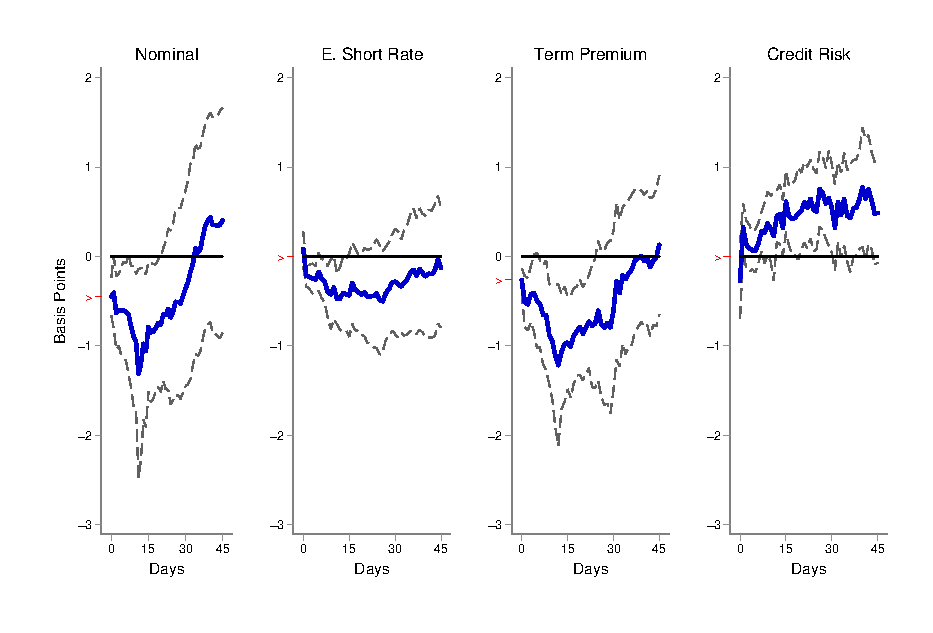
\includegraphics[trim={0cm 0cm 0cm 0cm},clip,height=0.45\textheight,width=0.85\linewidth]{../Figures/LPs/LagDep-FX/Path/EM/PathEMnomyptpphi120mPost.eps}
%\par\end{center}
%\end{figure}
%\vspace{-0.5cm}
%\begin{figure}[!htbp]
%\begin{center} % trim removes: left, down, right, top
%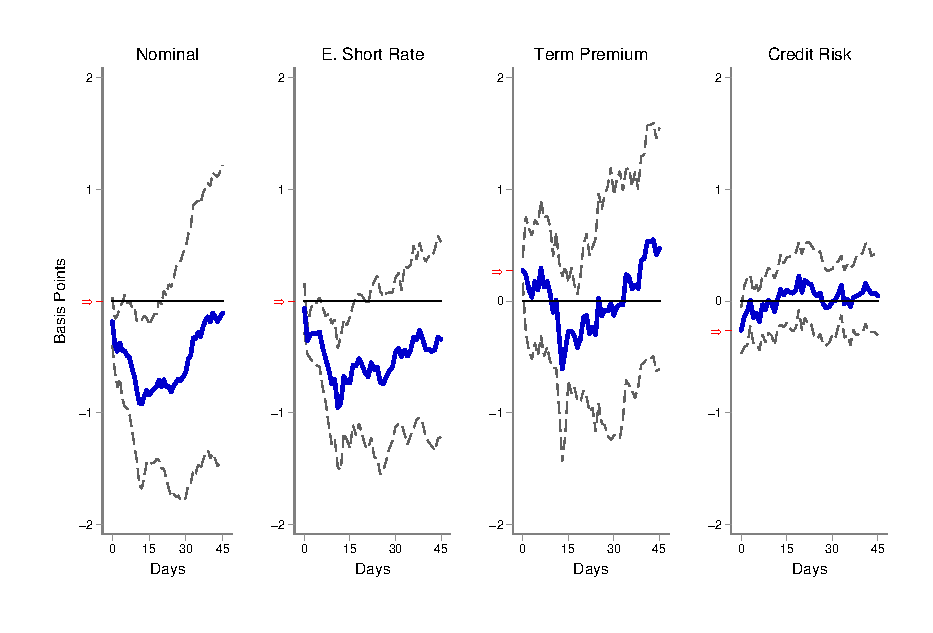
\includegraphics[trim={0cm 0cm 0cm 0.76cm},clip,height=0.45\textheight,width=0.85\linewidth]{../Figures/LPs/LagDep-FX/Path/EM/PathEMnomyptpphi24mPost.eps}
%\par\end{center}
%\end{figure}
%\begin{textblock*}{8mm}(10mm,30mm)
%\small \textbf{10Y}
%\end{textblock*}
%\begin{textblock*}{8mm}(10mm,65mm)
%\small \textbf{2Y}
%\end{textblock*}
%\begin{textblock*}{5cm}(1.07\textwidth,0.65\textheight)
%\hyperlink{FGUSpost}{\beamergotobutton{US}}
%\end{textblock*}
%\end{frame}
%\note{Following a FG shock, investors are relatively more attracted to invest LT in the US than in EM, so effect lasts longer in the US LT, which widens the spread b/w the nominal and synthetic YCs.}
%\note{After GFC, FG aim was to decline the LT USTP. This figure shows that FG surprises also lead to a decline in EM TP.}
%\note{Note that following the shock, the TP and the CRC move in opposite directions. Almost offsetting each other. Therefore, ignoring CR one would conclude that FG does not affect the EM TP.}
%\note{In relation to the YC channel, a FG is aimed at reducing the LT USTP and also reduces LT EMTP. Furhter, investors expect EM CB to reduce their policy rate in line with a risk spillover mechanism.}
%
%
%\begin{frame}[label=LSAPEM]
%\frametitle{Effects of Asset Purchase Easing on EM Yields}
%\begin{figure}[!htbp]
%\begin{center} % trim removes: left, down, right, top
%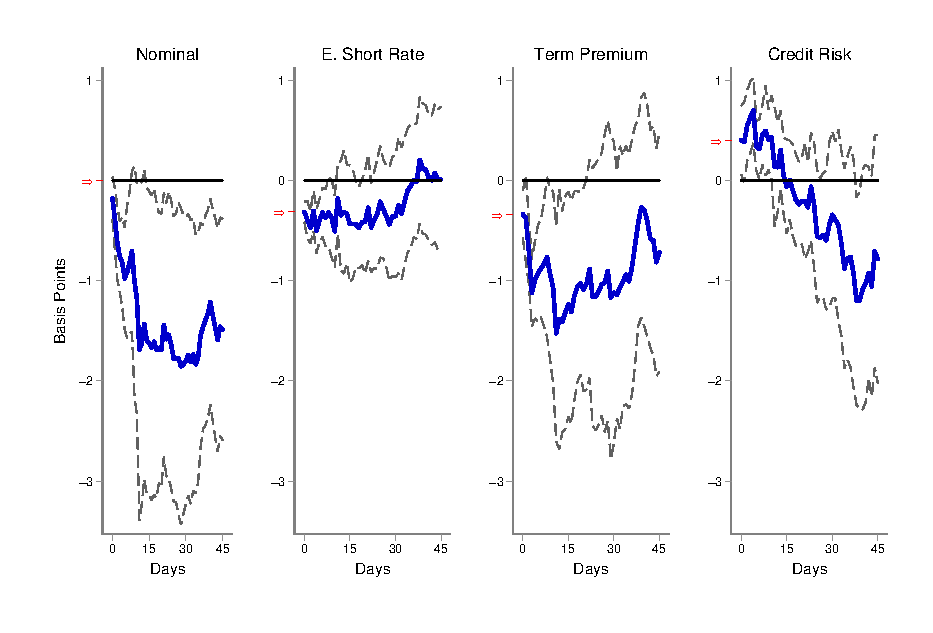
\includegraphics[trim={0cm 0cm 0cm 0cm},clip,height=0.45\textheight,width=0.85\linewidth]{../Figures/LPs/LagDep-FX/LSAP/EM/LSAPEMnomyptpphi120m.eps}
%\par\end{center}
%\end{figure}
%\vspace{-0.5cm}
%\begin{figure}[!htbp]
%\begin{center} % trim removes: left, down, right, top
%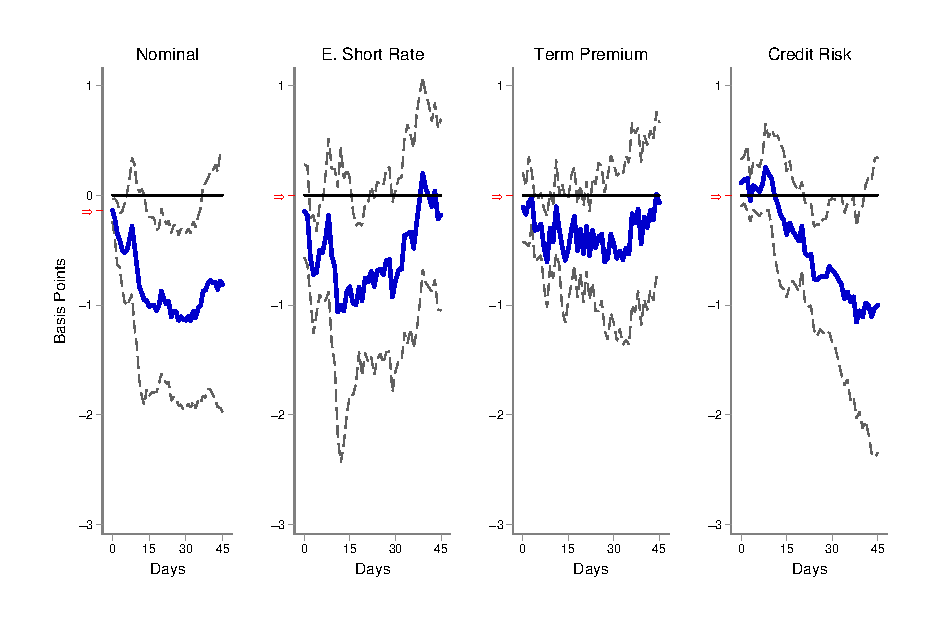
\includegraphics[trim={0cm 0cm 0cm 0.76cm},clip,height=0.45\textheight,width=0.85\linewidth]{../Figures/LPs/LagDep-FX/LSAP/EM/LSAPEMnomyptpphi24m.eps}
%\par\end{center}
%\end{figure}
%\begin{textblock*}{8mm}(10mm,30mm)
%\small \textbf{10Y}
%\end{textblock*}
%\begin{textblock*}{8mm}(10mm,65mm)
%\small \textbf{2Y}
%\end{textblock*}
%\begin{textblock*}{5cm}(1.07\textwidth,0.65\textheight)
%\hyperlink{LSAPUS}{\beamergotobutton{US}}
%\end{textblock*}
%\end{frame}
%\note{LSAP surprise flattens US and EM YCs.}
%\note{Effect at LT is larger than at ST but lasts longer in EM.}
%\note{Unlike a FG surprise, an LSAP shock incentivizes investors to invest in LT EM yields, reducing TP and CRC.}
%\note{Responses of LT TP and ST ESR also consistent with YC channel as with FG post-GFC.}
%\note{Evidence of a YC channel is present in responses to UMP.}
%
%
%\section{Conclusions}
%
%\begin{frame}
%\frametitle{Conclusions}
%
%\textbf{Three}-part decomposition of EM yields
%\begin{itemize}
%\item Average expected short rates \item Term premium \item \alert{Credit risk} compensation
%\end{itemize}
%
%U.S. monetary policy \textbf{spillovers} to EM yields
%\begin{enumerate}
%\item Responses are economically \alert{significant} yet \alert{delayed}
%\item Reassessment of policy rate expectations and repricing of \alert{risks}
%\item Evidence of a \alert{yield curve channel} since 2008
%\end{enumerate}
%
%\end{frame}
%\note{YC channel: EM monetary autonomy decreases along the yield curve and involves the credit risk compensation.}
%\note{To understand comovement, I propose a decomposition of EM yields.}
%\note{Extensions: nominal-real decompositions, jumps.}
%
%\begin{frame}[standout]
%Appendix
%\end{frame}
%
%\appendix
%
%\begin{frame}[label=CreditRating]
%\frametitle{Credit Risk in Local Currency Yields}
%\begin{center}
%	\includegraphics[width=0.95\textwidth,height=0.9\textheight]{../Figures/Slides/EM_LC_Ratings.png}
%\end{center}
%\begin{textblock*}{5cm}(0.87\textwidth,1.06\textheight)
%	\hyperlink{SovereignDefaults}{\beamerreturnbutton{Sovereigns Defaults}}
%\end{textblock*}
%\end{frame}
%\note{Few EM have a credit rating of A and more than 30 have a rating below investment grade of BBB.}
%\note{Figure: include Argentina, Brazil, China, Colombia, Egypt, Hungary, India, Indonesia, Lebanon, Malaysia, Mexico, Pakistan, Philippines, Poland, Qatar, Russia, Saudi Arabia, South Africa, Thailand, Turkey.}
%\note{A bond is considered investment grade if its credit rating is BBB- or higher. Bonds rated BB+ and below are considered to be speculative grade.}
%\note{Countries w/ AAA ratings: Australia, Canada,	Denmark, Finland, Germany, Luxembourg, Netherlands, Norway, Singapore, Sweden, Switzerland.}
%\note{BRL, TRY, ZAR don't have investment grade.}
%%\note{Credit risk broadly defined: (selective) default risk, currency convertibility risk, regulation risk, capital controls, jurisdiction risks, liquidity risk, sovereign restructurings.}
%
%
%\begin{frame}[label=AssetPricing]
%\frametitle{Asset Pricing}
%Under no arbitrage \(\rightarrow\) \(\exists\) a stochastic discount factor \(\SDF > 0\)
%\newline
%
%\(\SDF\) prices all nominal bonds under probability measure \(\Pmeasure\)
%\begin{equation*} \label{eq:uPzeroP}
	\PzeroP ,
\end{equation*}
%\vspace{1pt}
%
%\(\SDF\) \(\rightarrow\) \(\exists\) a risk-neutral measure \(\Qmeasure\) defined as % theoretical risk-neutral pricing
%\begin{equation*} \label{eq:uPzeroQ}
	\PzeroQ 
\end{equation*}
%
%\begin{textblock*}{3cm}(1\textwidth,1.05\textheight)
%	\hyperlink{ATSMsummary}{\beamerreturnbutton{Overview}}
%\end{textblock*}
%\end{frame}
%\note{Theoretical measure under which hypothetical investors are risk neutral that also serves to price bonds.}
%
%
%\begin{frame}[label=SDF]
%\frametitle{Stochastic Discount Factor}
%Stochastic discount factor
%\begin{equation*} \label{eq:uSDF}
	\eqSDF 
\end{equation*}
%
%Market prices of risk
%\begin{equation*} \label{eq:uRiskprice}
	\eqriskprice 
\end{equation*}
%
%One-period interest rate
%\begin{equation*} \label{eq:uShortRate}
	\eqshortrate 
\end{equation*}
%
%\begin{textblock*}{3cm}(1\textwidth,1.05\textheight)
%	\hyperlink{ATSMsummary}{\beamerreturnbutton{Overview}}
%\end{textblock*}
%
%\end{frame}
%\note{The model specifies the SDF as a function of the one-period interest rate and the market prices of risk, which are in turn affine functions of the pricing factors}
%\note{Market prices of risk control the transformation between the Q and P measures.}
%
%
%\begin{frame}[label=BondPrices]
%\frametitle{Bond Pricing}
%Pricing factors under \(\Pmeasure\) measure % physical
%\begin{equation*} \label{eq:uXvarsP}
	\eqXvarsFwdP
\end{equation*}
%
%Bond prices % is an exponentially affine function of the pricing factors
%\input{../Equations/uPaffine}
%
%\begin{center}
%\(\affineA = \mathcal{A}(\deltazero, \deltaone, \XmuP, \XPhiP, \XSigma, \tnr)\), \(\affineB = B(\deltaone, \XPhiP, \tnr)\) % \(\affineAP = - \frac{1}{\tnr} \affineA\), \(\affineBP = - \frac{1}{\tnr} \affineB\), 
%\end{center}
%
%Pricing factors under \(\Qmeasure\) measure % risk-neutral
%\begin{equation*} \label{eq:uXvarsQ}
	\eqXvarsFwdQ 
\end{equation*}
%
%\begin{textblock*}{3cm}(1\textwidth,1.05\textheight)
%\hyperlink{ATSMsummary}{\beamerreturnbutton{Overview}}
%\end{textblock*}
%\end{frame}
%\note{Pricing factors are assumed to follow a first-order VAR.}
%\note{These assumptions imply that the log price of the bond is an affine function of the pricing factors.}
%\note{Coefficients are functions of the model's parameters and the maturity of the bond.}
%\note{The structure for the market prices of risk implies that the dynamics of the pricing factors under the risk-neutral measure also follow a first-order VAR.}
%
%
%\begin{frame}[label=SvyAugModel]
%\frametitle{Survey-Augmented Model}
%
%Expected average short rate % under \(\Pmeasure\)
%\begin{equation*}
	\yZeroE = \affineAe + \affineBe \Xvars,
\end{equation*}
%\vspace{3pt}
%
%Forward rate from \(\tnr\) to \(\tnrfwd\) periods hence
%\begin{equation*}
	\yZeroEfwd = \affineAeFwd + \affineBeFwd \Xvars.
\end{equation*}
%
%\begin{textblock*}{3cm}(1\textwidth,1.05\textheight)
%	\hyperlink{ATSMsummary}{\beamerreturnbutton{Overview}}
%\end{textblock*}
%
%\end{frame}
%\note{To incorporate surveys in the model, the expected avg SR in the model is matched to the 5-year ahead implied forecast.}
%\note{The LT implied forecast is matched to the 5Y forward 5Y hence.}
%
%
%\begin{frame}[label=YldCBP]
%%	\frametitle{Components: Expected Future Short Rate}
%\begin{center}							% center the figure inside the minipage
%	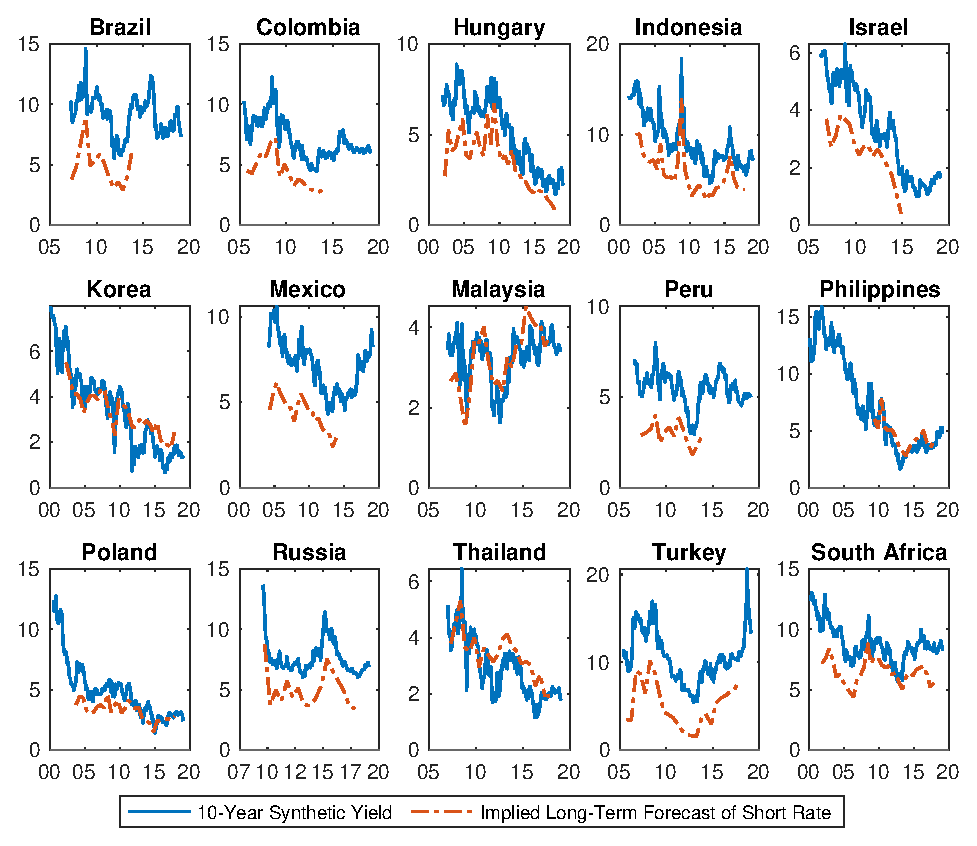
\includegraphics[trim={0cm 0cm 0cm 0cm},clip,height=0.95\textheight,width=\linewidth]{../Figures/Data/YLD10Y_CBP.eps} \\
%\end{center}
%\begin{textblock*}{5cm}(0.97\textwidth,1.05\textheight)
%	\hyperlink{SCBP}{\beamerreturnbutton{Survey Data}}
%\end{textblock*}
%\end{frame}
%\note{To see how sensible the implied forecasts for the short rate are, I compare them against the synthetic yields.}
%\note{In this figure forecasts in orange and synthetic yields in blue. You can see that the magnitudes are comparable.}
%\note{I compare them also against the real yields from TIPS and against an alternative approach using Taylor-rule type regressions, which also use forecasts for real GDP. The results are also comparable.}
%
%
%\begin{frame}[label=tpCI]
%%	\frametitle{Components: Term Premium}
%\begin{center}							% center the figure inside the minipage
%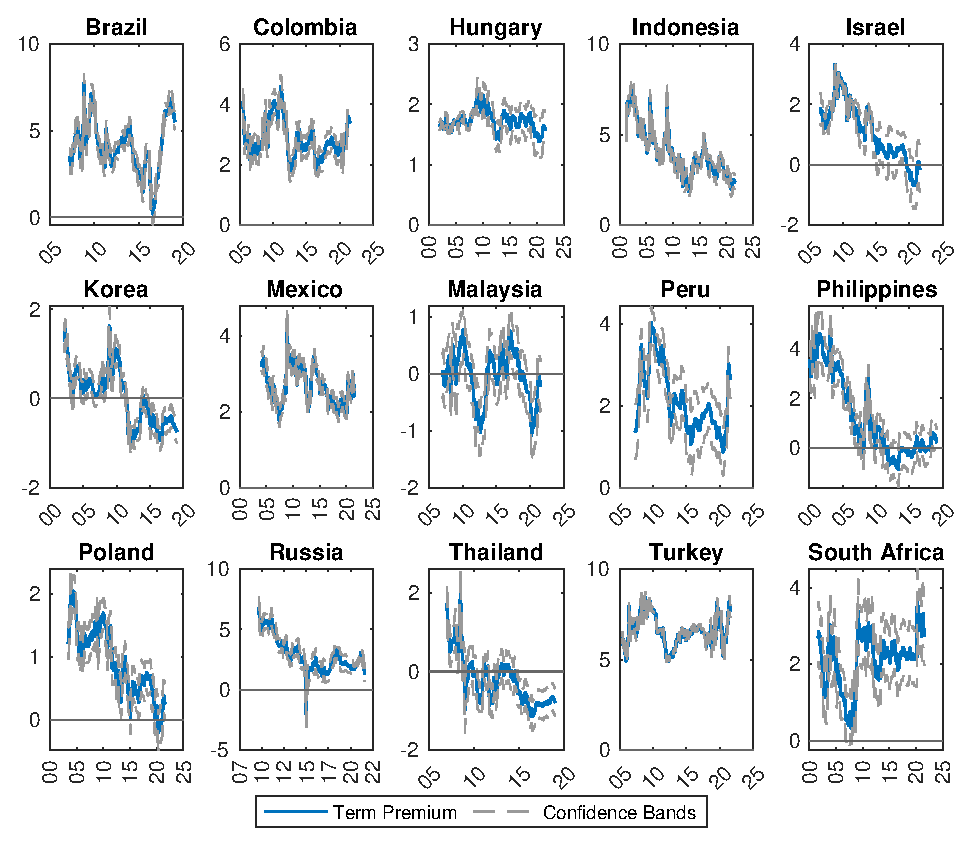
\includegraphics[trim={0cm 0cm 0cm 0cm},clip,height=0.95\textheight,width=\linewidth]{../Figures/Estimation/bsl_tp_CI_10y_V1.eps} \\
%\end{center}
%\begin{textblock*}{5cm}(0.97\textwidth,1.05\textheight)
%\hyperlink{YldDcmp}{\beamerreturnbutton{Decomposition}}
%\end{textblock*}
%\end{frame}
%\note{Survey-Based Term Premium Estimates}
%\note{EM TP are time-varying.}
%\note{Sensible TP estimates, mostly positive; fluctuate between 0\% and 5\%.}
%\note{Sometimes they comove.}
%
%\begin{frame}[label=crcCI]
%%\frametitle{Components: Credit Risk Compensation}
%\begin{center}							% center the figure inside the minipage
%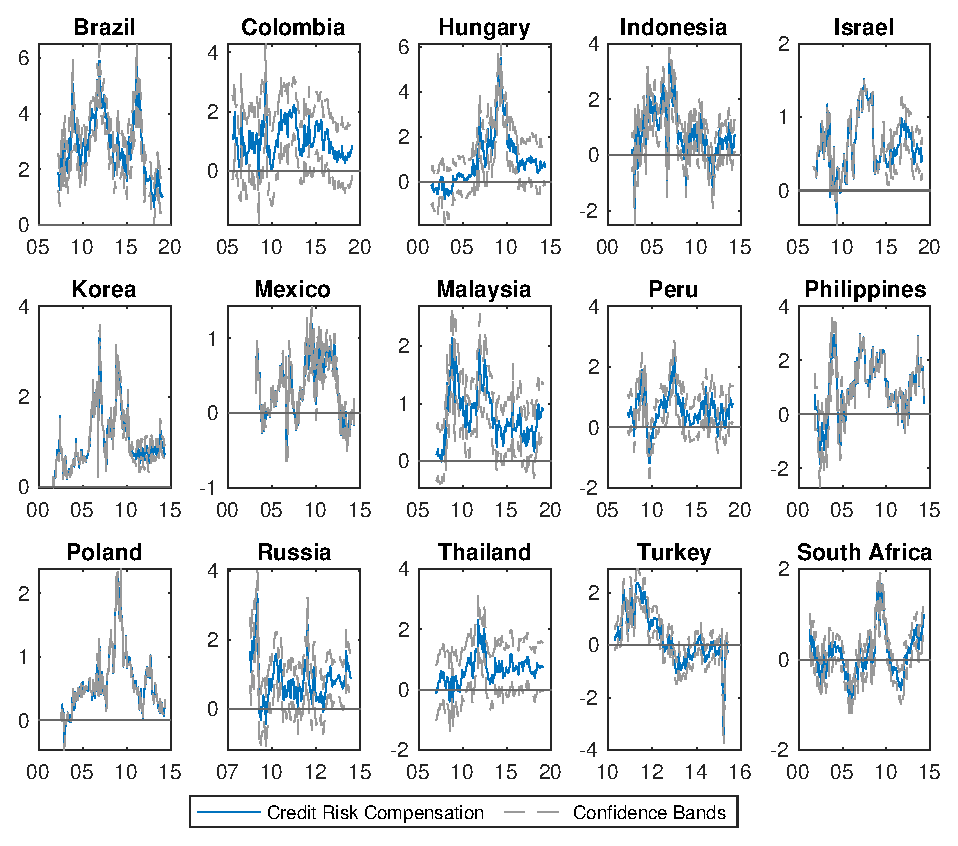
\includegraphics[trim={0cm 0cm 0cm 0cm},clip,height=0.95\textheight,width=\linewidth]{../Figures/Estimation/bsl_cr_CI_10y_V1.eps} \\
%\end{center}
%\begin{textblock*}{5cm}(0.97\textwidth,1.05\textheight)
%\hyperlink{YldDcmp}{\beamerreturnbutton{Decomposition}}
%\end{textblock*}
%\end{frame}
%
%%\begin{frame}[label=rrtLT]
%%%	\frametitle{Components: Expected Future Short Rate}
%%\begin{center}							% center the figure inside the minipage
%%	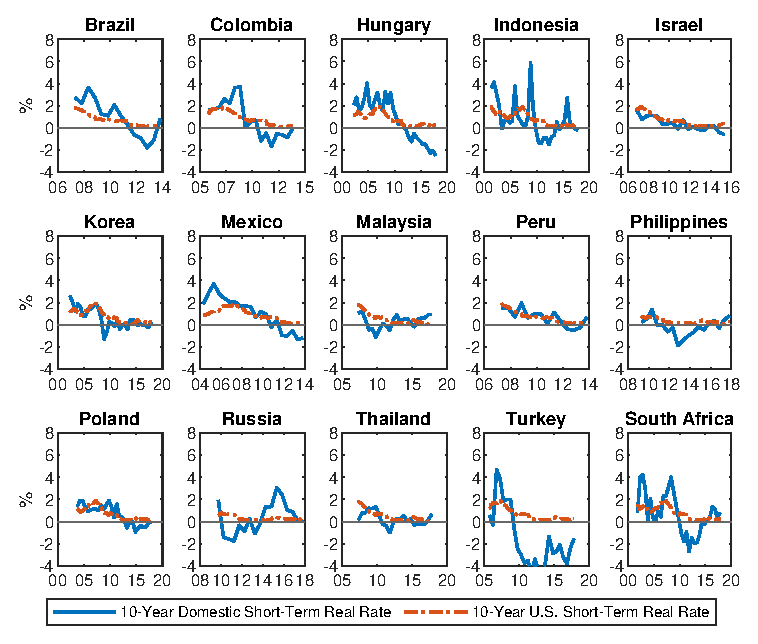
\includegraphics[trim={0cm 0cm 0cm 0cm},clip,height=1.05\textheight,width=\linewidth]{../Figures/Estimation/rrt_LTvsUSrrt.eps} \\
%%\end{center}
%%\begin{textblock*}{5cm}(0.95\textwidth,1.05\textheight)
%%	\hyperlink{yPscbp}{\beamerreturnbutton{Model vs Forecasts}}
%%\end{textblock*}
%%\end{frame}
%
%\begin{frame}[label=DYindex]
%\frametitle{EM Yields Comovement}
%\begin{figure}[!htbp]
%	\begin{center} % trim removes: left, down, right, top
%		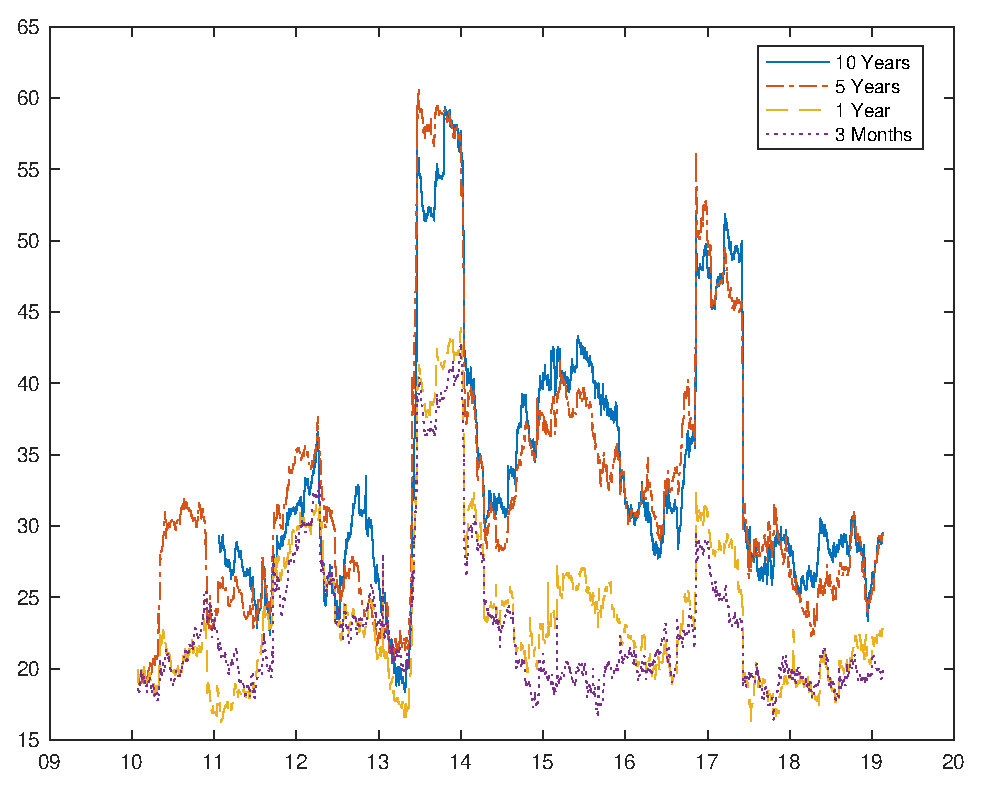
\includegraphics[trim={0cm 0cm 0cm 0cm},clip,height=0.8\textheight,width=0.85\linewidth]{../Figures/Estimation/dy_index_dn_data.eps}
%		\par\end{center}
%\end{figure}
%\begin{textblock*}{10cm}(45mm,83mm)
%	\footnotesize Connectedness Index \citep{DieboldYilmaz:2014}
%\end{textblock*}
%\begin{textblock*}{5cm}(1.02\textwidth,0.55\textheight)
%	\hyperlink{RollingCorr}{\beamergotobutton{Rolling Corr.}}
%\end{textblock*}
%\end{frame}
%
%%\begin{frame}[label=RollingCorr]
%%\frametitle{EM Yields Comovement}
%%\begin{figure}[!htbp]
%%\begin{center} % trim removes: left, down, right, top
%%	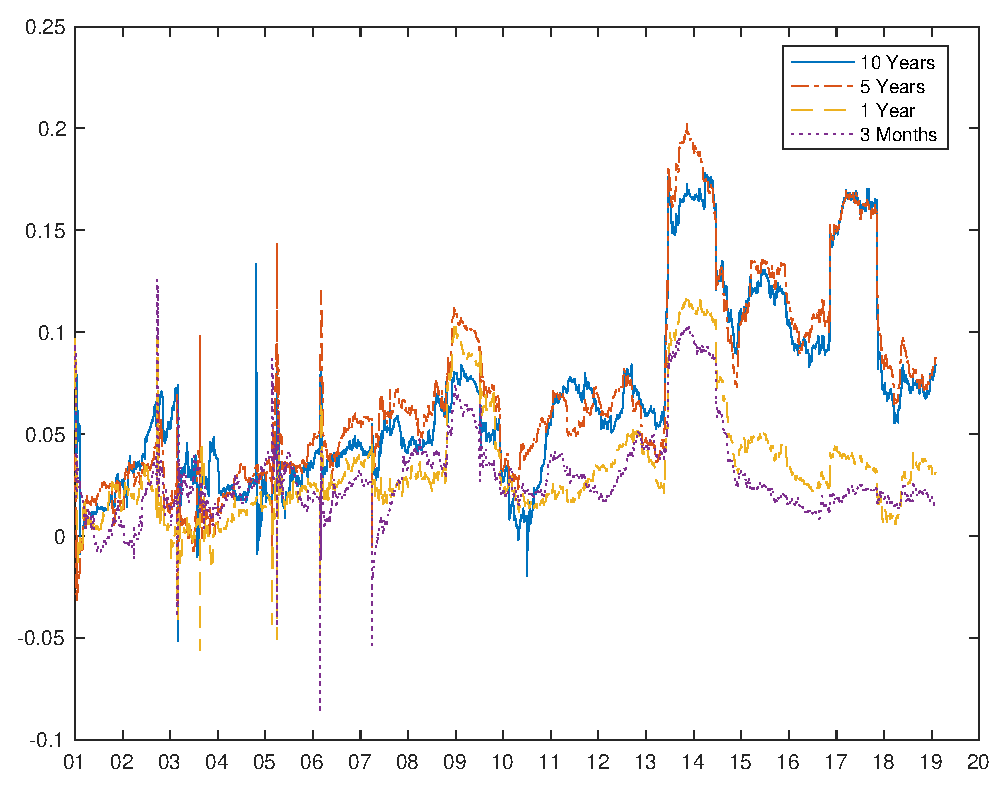
\includegraphics[trim={0cm 0cm 0cm 0cm},clip,height=0.8\textheight,width=0.85\linewidth]{../Figures/Estimation/rolling_dn_data.eps}
%%	\par\end{center}
%%\end{figure}
%%\begin{textblock*}{10cm}(67.5mm,83mm)
%%\footnotesize Rolling Correlations
%%\end{textblock*}
%%\begin{textblock*}{5cm}(1.02\textwidth,0.55\textheight)
%%\hyperlink{DYindex}{\beamergotobutton{D-Y Index}}
%%\end{textblock*}
%%\end{frame}
%
%
%\begin{frame}[label=Drivers10Y]
%%	\frametitle{EM Term Premium and Inflation Uncertainty}
%\vspace{-0.8cm}
%\begin{figure}[!htbp]
%	\begin{center} % trim removes: left, down, right, top
%		\includegraphics[trim={2cm 7.2cm 2cm 4cm},clip, width=0.95\textwidth,height=1.15\textheight]{../Tables/ycdcmp10y.pdf}
%		\par\end{center}
%\end{figure}
%\begin{textblock*}{5cm}(1.04\textwidth,0.09\textheight)
%	\hyperlink{Drivers10Y2Y}{\beamerreturnbutton{10Y \& 2Y}}
%\end{textblock*}
%\end{frame}
%
%
%\begin{frame}[label=Drivers2Y]
%%	\frametitle{EM Term Premium and Inflation Uncertainty}
%\vspace{-0.8cm}
%\begin{figure}[!htbp]
%\begin{center} % trim removes: left, down, right, top
%	\includegraphics[trim={2cm 7.2cm 2cm 4cm},clip, width=0.95\textwidth,height=1.15\textheight]{../Tables/ycdcmp2y.pdf}
%	\par\end{center}
%\end{figure}
%\begin{textblock*}{5cm}(1.04\textwidth,0.09\textheight)
%\hyperlink{Drivers10Y2Y}{\beamerreturnbutton{10Y \& 2Y}}
%\end{textblock*}
%\end{frame}
%\note{monetary autonomy is stronger at the short end than at the long end of the curve}
%\note{USTP and GFCy are more relevant for the long end than for the short end of EM YCs}
%
%
%\begin{frame}[label=TargetUS]
%\frametitle{Effects of Target Easing on U.S. Yields}
%\begin{figure}[!htbp]
%\begin{center} % trim removes: left, down, right, top
%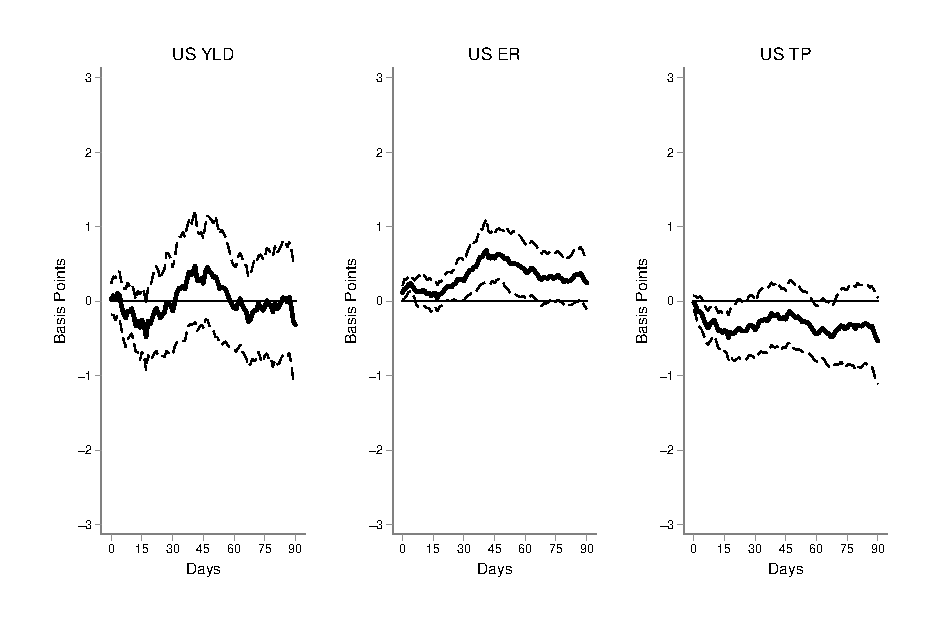
\includegraphics[trim={0cm 0cm 0cm 0cm},clip,height=0.45\textheight,width=0.85\linewidth]{../Figures/LPs/LagDep-FX/Target/US/DCMP/TargetUSDnomyptp120m.eps}
%\par\end{center}
%\end{figure}
%\vspace{-0.5cm}
%\begin{figure}[!htbp]
%\begin{center} % trim removes: left, down, right, top
%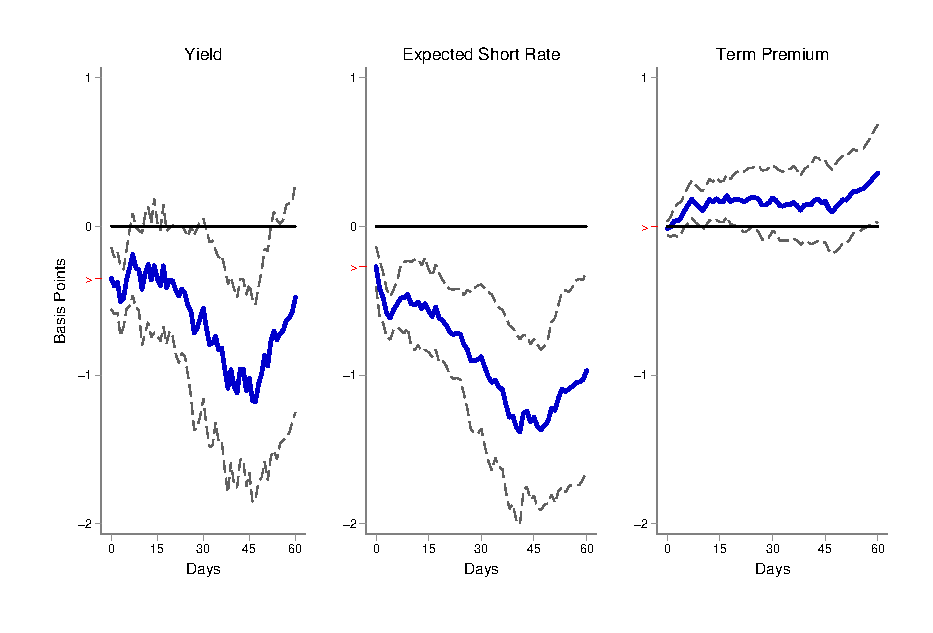
\includegraphics[trim={0cm 0cm 0cm 0.76cm},clip,height=0.45\textheight,width=0.85\linewidth]{../Figures/LPs/LagDep-FX/Target/US/DCMP/TargetUSDnomyptp24m.eps}
%\par\end{center}
%\end{figure}
%\begin{textblock*}{8mm}(10mm,30mm)
%\small \textbf{10Y}
%\end{textblock*}
%\begin{textblock*}{8mm}(10mm,65mm)
%\small \textbf{2Y}
%\end{textblock*}
%\begin{textblock*}{5cm}(1.07\textwidth,0.65\textheight)
%\hyperlink{TargetEM}{\beamerreturnbutton{EM}}
%\end{textblock*}
%\end{frame}
%
%\begin{frame}[label=FGUSpre]
%\frametitle{Effects of Forward Guidance Easing on U.S. Yields: Pre-GFC}
%\begin{figure}[!htbp]
%	\begin{center} % trim removes: left, down, right, top
%		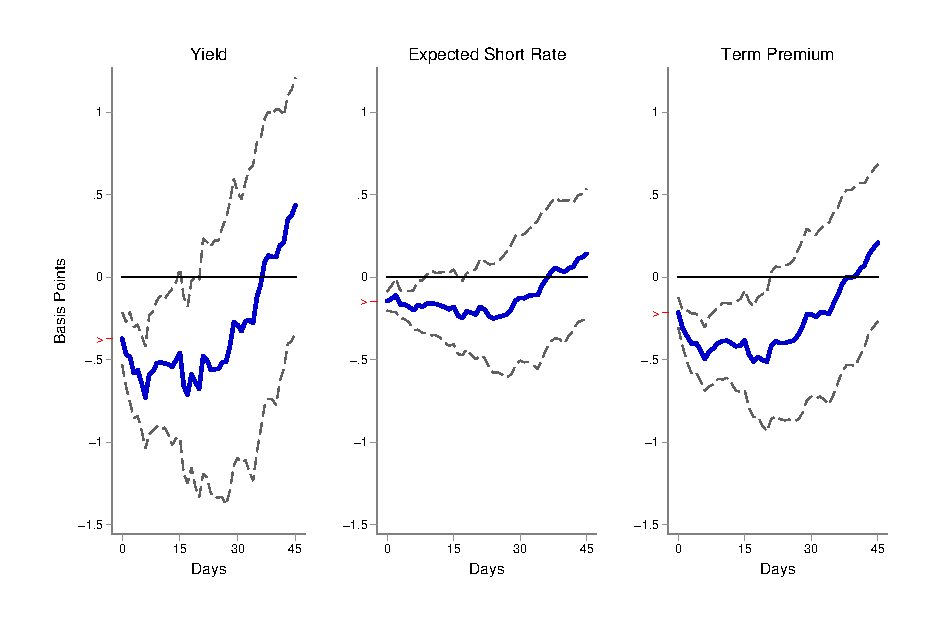
\includegraphics[trim={0cm 0cm 0cm 0cm},clip,height=0.45\textheight,width=0.85\linewidth]{../Figures/LPs/LagDep-FX/Path/US/DCMP/PathUSDnomyptp120mPre.eps}
%		\par\end{center}
%\end{figure}
%\vspace{-0.5cm}
%\begin{figure}[!htbp]
%	\begin{center} % trim removes: left, down, right, top
%		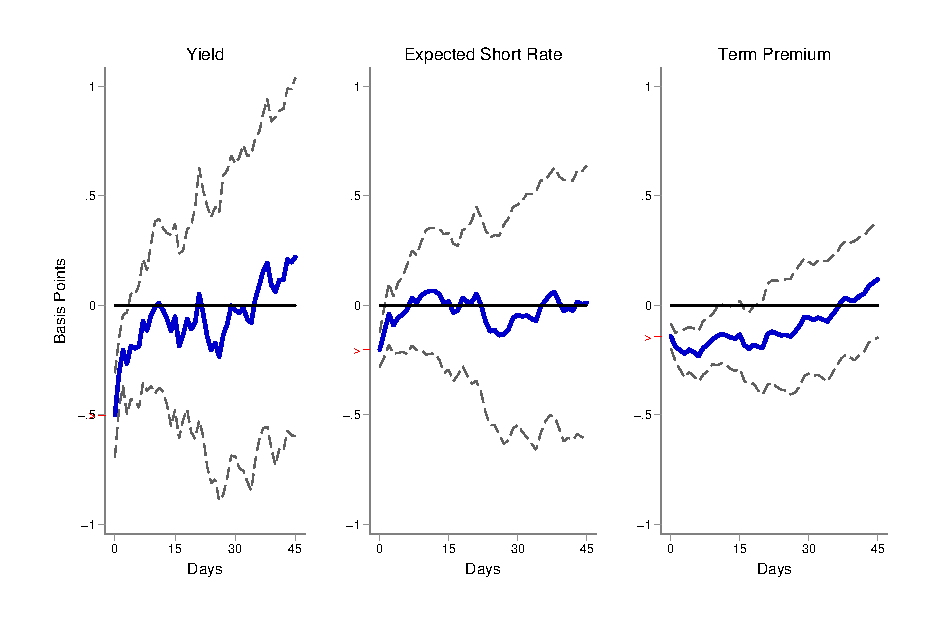
\includegraphics[trim={0cm 0cm 0cm 0.76cm},clip,height=0.45\textheight,width=0.85\linewidth]{../Figures/LPs/LagDep-FX/Path/US/DCMP/PathUSDnomyptp24mPre.eps}
%		\par\end{center}
%\end{figure}
%\begin{textblock*}{8mm}(10mm,30mm)
%	\small \textbf{10Y}
%\end{textblock*}
%\begin{textblock*}{8mm}(10mm,65mm)
%	\small \textbf{2Y}
%\end{textblock*}
%\begin{textblock*}{5cm}(1.07\textwidth,0.65\textheight)
%	\hyperlink{FGEMpre}{\beamerreturnbutton{EM}}
%\end{textblock*}
%\end{frame}
%
%\begin{frame}[label=FGUSpost]
%\frametitle{Effects of Forward Guidance Easing on U.S. Yields: Post-GFC}
%\begin{figure}[!htbp]
%\begin{center} % trim removes: left, down, right, top
%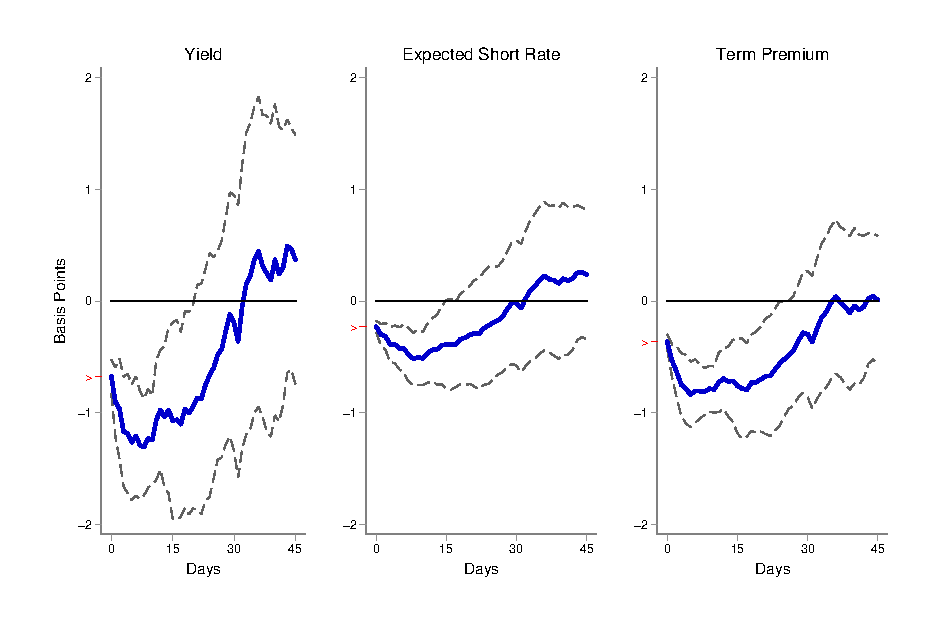
\includegraphics[trim={0cm 0cm 0cm 0cm},clip,height=0.45\textheight,width=0.85\linewidth]{../Figures/LPs/LagDep-FX/Path/US/DCMP/PathUSDnomyptp120mPost.eps}
%\par\end{center}
%\end{figure}
%\vspace{-0.5cm}
%\begin{figure}[!htbp]
%\begin{center} % trim removes: left, down, right, top
%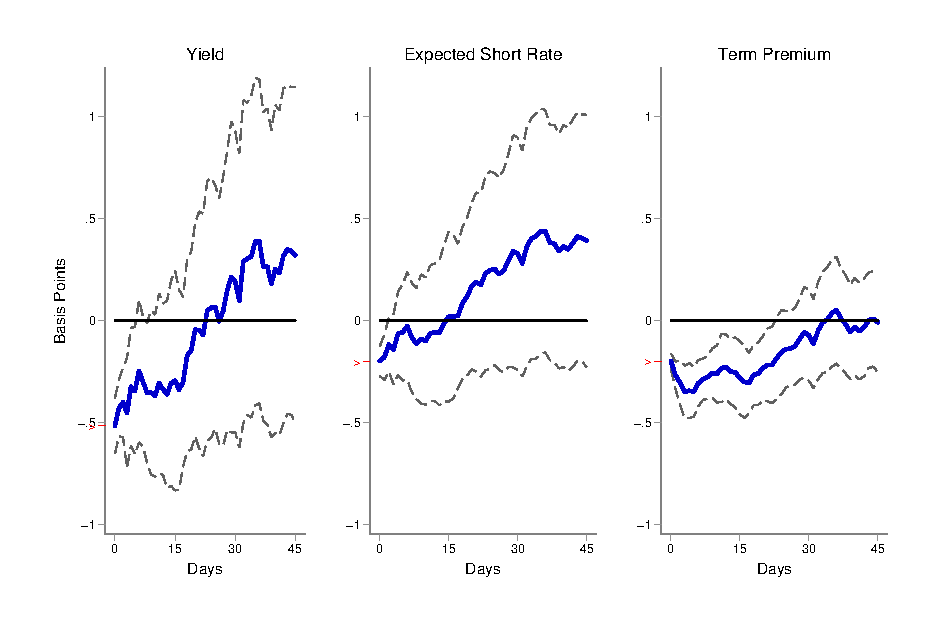
\includegraphics[trim={0cm 0cm 0cm 0.76cm},clip,height=0.45\textheight,width=0.85\linewidth]{../Figures/LPs/LagDep-FX/Path/US/DCMP/PathUSDnomyptp24mPost.eps}
%\par\end{center}
%\end{figure}
%\begin{textblock*}{8mm}(10mm,30mm)
%\small \textbf{10Y}
%\end{textblock*}
%\begin{textblock*}{8mm}(10mm,65mm)
%\small \textbf{2Y}
%\end{textblock*}
%\begin{textblock*}{5cm}(1.07\textwidth,0.65\textheight)
%\hyperlink{FGEMpost}{\beamerreturnbutton{EM}}
%\end{textblock*}
%\end{frame}
%
%\begin{frame}[label=LSAPUS]
%\frametitle{Effects of Asset Purchase Easing on U.S. Yields}
%\begin{figure}[!htbp]
%\begin{center} % trim removes: left, down, right, top
%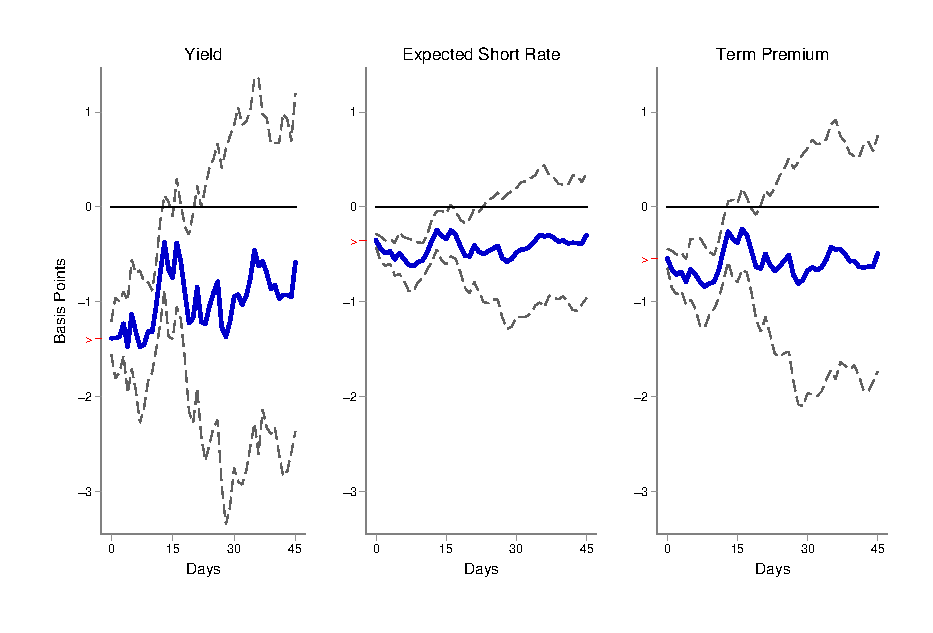
\includegraphics[trim={0cm 0cm 0cm 0cm},clip,height=0.45\textheight,width=0.85\linewidth]{../Figures/LPs/LagDep-FX/LSAP/US/DCMP/LSAPUSDnomyptp120m.eps}
%\par\end{center}
%\end{figure}
%\vspace{-0.5cm}
%\begin{figure}[!htbp]
%\begin{center} % trim removes: left, down, right, top
%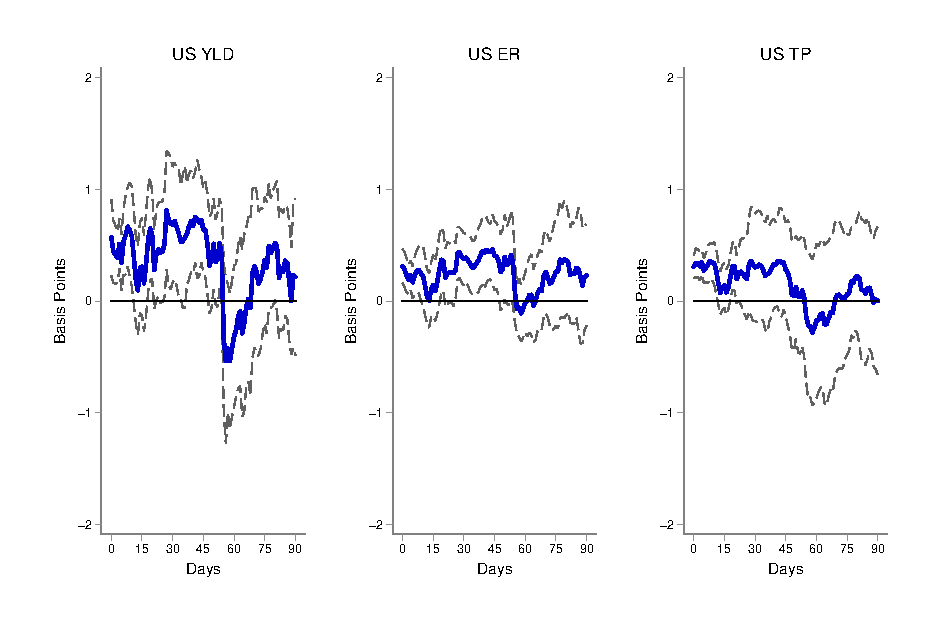
\includegraphics[trim={0cm 0cm 0cm 0.76cm},clip,height=0.45\textheight,width=0.85\linewidth]{../Figures/LPs/LagDep-FX/LSAP/US/DCMP/LSAPUSDnomyptp24m.eps}
%\par\end{center}
%\end{figure}
%\begin{textblock*}{8mm}(10mm,30mm)
%\small \textbf{10Y}
%\end{textblock*}
%\begin{textblock*}{8mm}(10mm,65mm)
%\small \textbf{2Y}
%\end{textblock*}
%\begin{textblock*}{5cm}(1.07\textwidth,0.65\textheight)
%\hyperlink{LSAPEM}{\beamerreturnbutton{EM}}
%\end{textblock*}
%\end{frame}

%---------------------------------------------------------------
% Sources
%---------------------------------------------------------------
% Tips in general
% https://en.wikibooks.org/wiki/LaTeX/Presentations
%https://tex.stackexchange.com/questions/12328/how-can-i-use-todonotes-with-beamer
% Insert links to slides
% https://latex.org/forum/viewtopic.php?t=4594
% Place button of link on slide
%https://tex.stackexchange.com/questions/50643/hyperlink-button-in-an-exact-position
% Make figures visible
%https://stackoverflow.com/questions/4683093/beamer-how-to-show-images-as-step-by-step-images
% Multicolumn and multirow
%https://tex.stackexchange.com/questions/156219/proper-centering-with-cmidrule-and-multi-row-and-column

% Metropolis
%http://mirrors.ibiblio.org/CTAN/macros/latex/contrib/beamer-contrib/themes/metropolis/doc/metropolistheme.pdf
%https://github.com/matze/mtheme

% Code for hyperlinks
%[label=corr_10yr]
%\begin{textblock*}{3cm}(.9\textwidth,-.5\textheight)
%	\hyperlink{corr_10yr}{\beamergotobutton{10-Year TP}}
%\end{textblock*}
%
%\begin{textblock*}{3cm}(.9\textwidth,-.5\textheight)
%	\hyperlink{corr_10yr}{\beamerreturnbutton{10-Year TP}}
%\end{textblock*}

% Two-column frame template
%http://felix11h.github.io/blog/beamer-two-col



%\begin{frame}[allowframebreaks]{References}
\begin{frame}<presentation:0>
\bibliographystyle{abbrvnat} 
\bibliography{../../../References/library}
\end{frame}

\end{document}